% Finished mode.
% \documentclass[nocolor]{article}
% \documentclass{article}

% Draft mode.
% \documentclass[working,nocolor]{article}
\documentclass[working]{article}

%%%%%%%%%%%%%%%%%%%%%%%%%%%%%%%%%%%%%%%%%%%%%%%%%%%%%%%%%%%%%%%%%%%%%%%%%%%%%%%
%                                Basic Packages                               %
%%%%%%%%%%%%%%%%%%%%%%%%%%%%%%%%%%%%%%%%%%%%%%%%%%%%%%%%%%%%%%%%%%%%%%%%%%%%%%%

% Gives us multiple colors.
\usepackage[usenames,dvipsnames,pdftex]{xcolor}
% Lets us style link colors.
\usepackage{hyperref}
% Lets us import images and graphics.
\usepackage{graphicx}
% Lets us use figures in floating environments.
\usepackage{float}
% Lets us create multiple columns.
\usepackage{multicol}
% Gives us better math syntax.
\usepackage{amsmath,amsfonts,mathtools,amsthm,amssymb}
% Lets us strikethrough text.
\usepackage{cancel}
% Lets us edit the caption of a figure.
\usepackage{caption}
% Lets us import pdf directly in our tex code.
\usepackage{pdfpages}
% Lets us do algorithm stuff.
\usepackage[ruled,vlined,linesnumbered]{algorithm2e}
% Use a smiley face for our qed symbol.
\usepackage{tikzsymbols}

\usepackage{tikz-3dplot}
\usepackage[british]{datetime2}

\usetikzlibrary{automata,positioning}
\tikzset{
  vlak/.style={fill=lightgray!80,draw=none,opacity=1},
  obj/.style={fill=lightgray,draw=none},
  opp/.style={fill=lightgray,opacity=0.6,draw=none},
  rand/.style={thick,draw=gray},
  vector/.style={>=stealth',draw=black,line width=0.55pt}
  }
  \tdplotsetmaincoords{75}{140}

\renewcommand\qedsymbol{$\Laughey$}

\def\class{article}


%%%%%%%%%%%%%%%%%%%%%%%%%%%%%%%%%%%%%%%%%%%%%%%%%%%%%%%%%%%%%%%%%%%%%%%%%%%%%%%
%                                Basic Settings                               %
%%%%%%%%%%%%%%%%%%%%%%%%%%%%%%%%%%%%%%%%%%%%%%%%%%%%%%%%%%%%%%%%%%%%%%%%%%%%%%%

%%%%%%%%%%%%%
%  Symbols  %
%%%%%%%%%%%%%

\let\implies\Rightarrow
\let\impliedby\Leftarrow
\let\iff\Leftrightarrow
\let\epsilon\varepsilon

%%%%%%%%%%%%
%  Tables  %
%%%%%%%%%%%%

\setlength{\tabcolsep}{5pt}
\renewcommand\arraystretch{1.5}

%%%%%%%%%%%%%%
%  SI Unitx  %
%%%%%%%%%%%%%%

\usepackage{siunitx}
\sisetup{locale = FR}

%%%%%%%%%%
%  TikZ  %
%%%%%%%%%%

\usepackage[framemethod=TikZ]{mdframed}
\usepackage{tikz}
\usepackage{tikz-cd}
\usepackage{tikzsymbols}

\usetikzlibrary{intersections, angles, quotes, calc, positioning}
\usetikzlibrary{arrows.meta}

\tikzset{
  force/.style={thick, {Circle[length=2pt]}-stealth, shorten <=-1pt}
}

%%%%%%%%%%%%%%%
%  PGF Plots  %
%%%%%%%%%%%%%%%

\usepackage{pgfplots}
\pgfplotsset{compat=1.13}

%%%%%%%%%%%%%%%%%%%%%%%
%  Center Title Page  %
%%%%%%%%%%%%%%%%%%%%%%%

\usepackage{titling}
\renewcommand\maketitlehooka{\null\mbox{}\vfill}
\renewcommand\maketitlehookd{\vfill\null}

%%%%%%%%%%%%%%%%%%%%%%%%%%%%%%%%%%%%%%%%%%%%%%%%%%%%%%%
%  Create a grey background in the middle of the PDF  %
%%%%%%%%%%%%%%%%%%%%%%%%%%%%%%%%%%%%%%%%%%%%%%%%%%%%%%%

\usepackage{eso-pic}
\newcommand\definegraybackground{
  \definecolor{reallylightgray}{HTML}{FAFAFA}
  \AddToShipoutPicture{
    \ifthenelse{\isodd{\thepage}}{
      \AtPageLowerLeft{
        \put(\LenToUnit{\dimexpr\paperwidth-222pt},0){
          \color{reallylightgray}\rule{222pt}{297mm}
        }
      }
    }
    {
      \AtPageLowerLeft{
        \color{reallylightgray}\rule{222pt}{297mm}
      }
    }
  }
}

%%%%%%%%%%%%%%%%%%%%%%%%
%  Modify Links Color  %
%%%%%%%%%%%%%%%%%%%%%%%%

\hypersetup{
  % Enable highlighting links.
  colorlinks,
  % Change the color of links to blue.
  linkcolor=blue,
  % Change the color of citations to black.
  citecolor={black},
  % Change the color of url's to blue with some black.
  urlcolor={blue!80!black}
}

%%%%%%%%%%%%%%%%%%
% Fix WrapFigure %
%%%%%%%%%%%%%%%%%%

\newcommand{\wrapfill}{\par\ifnum\value{WF@wrappedlines}>0
    \parskip=0pt
    \addtocounter{WF@wrappedlines}{-1}%
    \null\vspace{\arabic{WF@wrappedlines}\baselineskip}%
    \WFclear
\fi}

%%%%%%%%%%%%%%%%%
% Multi Columns %
%%%%%%%%%%%%%%%%%

\let\multicolmulticols\multicols
\let\endmulticolmulticols\endmulticols

\RenewDocumentEnvironment{multicols}{mO{}}
{%
  \ifnum#1=1
    #2%
  \else % More than 1 column
    \multicolmulticols{#1}[#2]
  \fi
}
{%
  \ifnum#1=1
\else % More than 1 column
  \endmulticolmulticols
\fi
}

\newlength{\thickarrayrulewidth}
\setlength{\thickarrayrulewidth}{5\arrayrulewidth}


%%%%%%%%%%%%%%%%%%%%%%%%%%%%%%%%%%%%%%%%%%%%%%%%%%%%%%%%%%%%%%%%%%%%%%%%%%%%%%%
%                           School Specific Commands                          %
%%%%%%%%%%%%%%%%%%%%%%%%%%%%%%%%%%%%%%%%%%%%%%%%%%%%%%%%%%%%%%%%%%%%%%%%%%%%%%%

%%%%%%%%%%%%%%%%%%%%%%%%%%%
%  Initiate New Counters  %
%%%%%%%%%%%%%%%%%%%%%%%%%%%

\newcounter{lecturecounter}

%%%%%%%%%%%%%%%%%%%%%%%%%%
%  Helpful New Commands  %
%%%%%%%%%%%%%%%%%%%%%%%%%%

\makeatletter

\newcommand\resetcounters{
  % Reset the counters for subsection, subsubsection and the definition
  % all the custom environments.
  \setcounter{subsection}{0}
  \setcounter{subsubsection}{0}
  \setcounter{paragraph}{0}
  \setcounter{subparagraph}{0}
  \setcounter{theorem}{0}
  \setcounter{claim}{0}
  \setcounter{corollary}{0}
  \setcounter{lemma}{0}
  \setcounter{exercise}{0}

  \@ifclasswith\class{nocolor}{
    \setcounter{definition}{0}
  }{}
}

%%%%%%%%%%%%%%%%%%%%%
%  Lecture Command  %
%%%%%%%%%%%%%%%%%%%%%

\usepackage{xifthen}

% EXAMPLE:
% 1. \lesson{Oct 17 2022 Mon (08:46:48)}{Lecture Title}
% 2. \lesson[4]{Oct 17 2022 Mon (08:46:48)}{Lecture Title}
% 3. \lesson{Oct 17 2022 Mon (08:46:48)}{}
% 4. \lesson[4]{Oct 17 2022 Mon (08:46:48)}{}
% Parameters:
% 1. (Optional) Lesson number.
% 2. Time and date of lecture.
% 3. Lecture Title.
\def\@lesson{}
\newcommand\lesson[3][\arabic{lecturecounter}]{
  % Add 1 to the lecture counter.
  \addtocounter{lecturecounter}{1}

  % Set the section number to the lecture counter.
  \setcounter{section}{#1}
  \renewcommand\thesubsection{#1.\arabic{subsection}}

  % Reset the counters.
  \resetcounters

  % Check if user passed the lecture title or not.
  \ifthenelse{\isempty{#3}}{
    \def\@lesson{Lecture \arabic{lecturecounter}}
  }{
    \def\@lesson{Lecture \arabic{lecturecounter}: #3}
  }

  % Display the information like the following:
  %                                                  Oct 17 2022 Mon (08:49:10)
  % ---------------------------------------------------------------------------
  % Lecture 1: Lecture Title
  \hfill\small{#2}
  \hrule
  \vspace*{-0.3cm}
  \section*{\@lesson}
  \addcontentsline{toc}{section}{\@lesson}
}

%%%%%%%%%%%%%%%%%%%%
%  Import Figures  %
%%%%%%%%%%%%%%%%%%%%

\usepackage{import}
\pdfminorversion=7

% EXAMPLE:
% 1. \incfig{limit-graph}
% 2. \incfig[0.4]{limit-graph}
% Parameters:
% 1. The figure name. It should be located in figures/NAME.tex_pdf.
% 2. (Optional) The width of the figure. Example: 0.5, 0.35.
\newcommand\incfig[2][1]{%
  \def\svgwidth{#1\columnwidth}
  \import{./figures/}{#2.pdf_tex}
}

\begingroup\expandafter\expandafter\expandafter\endgroup
\expandafter\ifx\csname pdfsuppresswarningpagegroup\endcsname\relax
\else
  \pdfsuppresswarningpagegroup=1\relax
\fi

%%%%%%%%%%%%%%%%%
% Fancy Headers %
%%%%%%%%%%%%%%%%%

\usepackage{fancyhdr}

% Force a new page.
\newcommand\forcenewpage{\clearpage\mbox{~}\clearpage\newpage}

% This command makes it easier to manage my headers and footers.
\newcommand\createintro{
  % Use roman page numbers (e.g. i, v, vi, x, ...)
  \pagenumbering{roman}

  % Display the page style.
  \maketitle
  % Make the title pagestyle empty, meaning no fancy headers and footers.
  \thispagestyle{empty}
  % Create a newpage.
  \newpage

  % Input the intro.tex page if it exists.
  \IfFileExists{intro.tex}{ % If the intro.tex file exists.
    % Input the intro.tex file.
    Lecture notes from the 2023 undergraduate course Quantum Computing, given by Professor James D Kiper at Miami University at Benton Hall in the academic year 2022-2023. This course covers introductory quantum computing concepts. Credit for the material in these notes is due to Professor James D Kiper, while the structure is loosely taken from the in-class lectures. The credit for the typesetting is my own.

\textit{Disclaimer:} This document will inevitably contain some mistakes–both simple typos and legitimate errors. Keep in mind that these are the notes of an undergraduate student in the process of learning the material, so take what you read with a grain of salt. If you find mistakes and feel like telling me, I will be grateful and happy to hear from you, even for the most trivial of errors. You can reach me by email, in English, at \href{mailto:sayahie@miamioh.edu}{sayahie@miamioh.edu}.

    % Make the pagestyle fancy for the intro.tex page.
    \pagestyle{fancy}

    % Remove the line for the header.
    \renewcommand\headrulewidth{0pt}

    % Remove all header stuff.
    \fancyhead{}

    % Add stuff for the footer in the center.
    \fancyfoot[C]{
      \textit{For more notes like this, visit
      \href{\linktootherpages}{\shortlinkname}}. \\
      \vspace{0.1cm}
      \hrule
      \vspace{0.1cm}
      \@author, \\
      \term: \academicyear, \\
      Last Update: \@date, \\
      \faculty
    }
  }{ % If the intro.tex file doesn't exist.
    % Force a \newpageage.
    \forcenewpage
  }

  % Create a new page.
  \newpage

  % Remove the center stuff we did above, and replace it with just the page
  % number, which is still in roman numerals.
  \fancyfoot[C]{\thepage}
  % Add the table of contents.
  \tableofcontents
  % Force a new page.
  \forcenewpage

  % Move the page numberings back to arabic, from roman numerals.
  \pagenumbering{arabic}
  % Set the page number to 1.
  \setcounter{page}{1}

  % Add the header line back.
  \renewcommand\headrulewidth{0.4pt}
  % In the top right, add the lecture title.
  \fancyhead[R]{\@lesson}
  % In the top left, add the author name.
  \fancyhead[L]{\@author}
  % In the bottom center, add the page.
  \fancyfoot[C]{\thepage}
  % Add a nice gray background in the middle of all the upcoming pages.
  % \definegraybackground
}

\makeatother


%%%%%%%%%%%%%%%%%%%%%%%%%%%%%%%%%%%%%%%%%%%%%%%%%%%%%%%%%%%%%%%%%%%%%%%%%%%%%%%
%                               Custom Commands                               %
%%%%%%%%%%%%%%%%%%%%%%%%%%%%%%%%%%%%%%%%%%%%%%%%%%%%%%%%%%%%%%%%%%%%%%%%%%%%%%%

%%%%%%%%%%%%
%  Circle  %
%%%%%%%%%%%%

\newcommand*\circled[1]{\tikz[baseline=(char.base)]{
  \node[shape=circle,draw,inner sep=1pt] (char) {#1};}
}

%%%%%%%%%%%%%%%%%%%
%  Todo Commands  %
%%%%%%%%%%%%%%%%%%%

\usepackage{xargs}
\usepackage[colorinlistoftodos]{todonotes}

\makeatletter

\@ifclasswith\class{working}{
  \newcommandx\unsure[2][1=]{\todo[linecolor=red,backgroundcolor=red!25,bordercolor=red,#1]{#2}}
  \newcommandx\change[2][1=]{\todo[linecolor=blue,backgroundcolor=blue!25,bordercolor=blue,#1]{#2}}
  \newcommandx\info[2][1=]{\todo[linecolor=OliveGreen,backgroundcolor=OliveGreen!25,bordercolor=OliveGreen,#1]{#2}}
  \newcommandx\improvement[2][1=]{\todo[linecolor=Plum,backgroundcolor=Plum!25,bordercolor=Plum,#1]{#2}}

  \newcommand\listnotes{
    \newpage
    \listoftodos[Notes]
  }
}{
  \newcommandx\unsure[2][1=]{}
  \newcommandx\change[2][1=]{}
  \newcommandx\info[2][1=]{}
  \newcommandx\improvement[2][1=]{}

  \newcommand\listnotes{}
}

\makeatother

%%%%%%%%%%%%%
%  Correct  %
%%%%%%%%%%%%%

% EXAMPLE:
% 1. \correct{INCORRECT}{CORRECT}
% Parameters:
% 1. The incorrect statement.
% 2. The correct statement.
\definecolor{correct}{HTML}{009900}
\newcommand\correct[2]{{\color{red}{#1 }}\ensuremath{\to}{\color{correct}{ #2}}}


%%%%%%%%%%%%%%%%%%%%%%%%%%%%%%%%%%%%%%%%%%%%%%%%%%%%%%%%%%%%%%%%%%%%%%%%%%%%%%%
%                                 Environments                                %
%%%%%%%%%%%%%%%%%%%%%%%%%%%%%%%%%%%%%%%%%%%%%%%%%%%%%%%%%%%%%%%%%%%%%%%%%%%%%%%

\usepackage{varwidth}
\usepackage{thmtools}
\usepackage[most,many,breakable]{tcolorbox}

\tcbuselibrary{theorems,skins,hooks}
\usetikzlibrary{arrows,calc,shadows.blur}

%%%%%%%%%%%%%%%%%%%
%  Define Colors  %
%%%%%%%%%%%%%%%%%%%

\definecolor{myblue}{RGB}{45, 111, 177}
\definecolor{mygreen}{RGB}{56, 140, 70}
\definecolor{myred}{RGB}{199, 68, 64}
\definecolor{mypurple}{RGB}{197, 92, 212}

\definecolor{definition}{HTML}{228b22}
\definecolor{theorem}{HTML}{00007B}
\definecolor{example}{HTML}{2A7F7F}
\definecolor{definition}{HTML}{228b22}
\definecolor{prop}{HTML}{191971}
\definecolor{lemma}{HTML}{983b0f}
\definecolor{exercise}{HTML}{88D6D1}

\colorlet{definition}{mygreen!85!black}
\colorlet{claim}{mygreen!85!black}
\colorlet{corollary}{mypurple!85!black}
\colorlet{proof}{theorem}

%%%%%%%%%%%%%%%%%%%%%%%%%%%%%%%%%%%%%%%%%%%%%%%%%%%%%%%%%
%  Create Environments Styles Based on Given Parameter  %
%%%%%%%%%%%%%%%%%%%%%%%%%%%%%%%%%%%%%%%%%%%%%%%%%%%%%%%%%

\mdfsetup{skipabove=1em,skipbelow=0em}

%%%%%%%%%%%%%%%%%%%%%%
%  Helpful Commands  %
%%%%%%%%%%%%%%%%%%%%%%

% EXAMPLE:
% 1. \createnewtheoremstyle{thmdefinitionbox}{}{}
% 2. \createnewtheoremstyle{thmtheorembox}{}{}
% 3. \createnewtheoremstyle{thmproofbox}{qed=\qedsymbol}{
%       rightline=false, topline=false, bottomline=false
%    }
% Parameters:
% 1. Theorem name.
% 2. Any extra parameters to pass directly to declaretheoremstyle.
% 3. Any extra parameters to pass directly to mdframed.
\newcommand\createnewtheoremstyle[3]{
  \declaretheoremstyle[
  headfont=\bfseries\sffamily, bodyfont=\normalfont, #2,
  mdframed={
    #3,
  },
  ]{#1}
}

% EXAMPLE:
% 1. \createnewcoloredtheoremstyle{thmdefinitionbox}{definition}{}{}
% 2. \createnewcoloredtheoremstyle{thmexamplebox}{example}{}{
%       rightline=true, leftline=true, topline=true, bottomline=true
%     }
% 3. \createnewcoloredtheoremstyle{thmproofbox}{proof}{qed=\qedsymbol}{backgroundcolor=white}
% Parameters:
% 1. Theorem name.
% 2. Color of theorem.
% 3. Any extra parameters to pass directly to declaretheoremstyle.
% 4. Any extra parameters to pass directly to mdframed.
\newcommand\createnewcoloredtheoremstyle[4]{
  \declaretheoremstyle[
  headfont=\bfseries\sffamily\color{#2}, bodyfont=\normalfont, #3,
  mdframed={
    linewidth=2pt,
    rightline=false, leftline=true, topline=false, bottomline=false,
    linecolor=#2, backgroundcolor=#2!5, #4,
  },
  ]{#1}
}

%%%%%%%%%%%%%%%%%%%%%%%%%%%%%%%%%%%
%  Create the Environment Styles  %
%%%%%%%%%%%%%%%%%%%%%%%%%%%%%%%%%%%

\makeatletter
\@ifclasswith\class{nocolor}{
  % Environments without color.

  \createnewtheoremstyle{thmdefinitionbox}{}{}
  \createnewtheoremstyle{thmtheorembox}{}{}
  \createnewtheoremstyle{thmexamplebox}{}{}
  \createnewtheoremstyle{thmclaimbox}{}{}
  \createnewtheoremstyle{thmcorollarybox}{}{}
  \createnewtheoremstyle{thmpropbox}{}{}
  \createnewtheoremstyle{thmlemmabox}{}{}
  \createnewtheoremstyle{thmexercisebox}{}{}
  \createnewtheoremstyle{thmdefinitionbox}{}{}
  \createnewtheoremstyle{thmquestionbox}{}{}
  \createnewtheoremstyle{thmsolutionbox}{}{}

  \createnewtheoremstyle{thmproofbox}{qed=\qedsymbol}{}
  \createnewtheoremstyle{thmexplanationbox}{}{}
}{
  % Environments with color.

  \createnewcoloredtheoremstyle{thmdefinitionbox}{definition}{}{}
  \createnewcoloredtheoremstyle{thmtheorembox}{theorem}{}{}
  \createnewcoloredtheoremstyle{thmexamplebox}{example}{}{
    rightline=true, leftline=true, topline=true, bottomline=true
  }
  \createnewcoloredtheoremstyle{thmclaimbox}{claim}{}{}
  \createnewcoloredtheoremstyle{thmcorollarybox}{corollary}{}{}
  \createnewcoloredtheoremstyle{thmpropbox}{prop}{}{}
  \createnewcoloredtheoremstyle{thmlemmabox}{lemma}{}{}
  \createnewcoloredtheoremstyle{thmexercisebox}{exercise}{}{}

  \createnewcoloredtheoremstyle{thmproofbox}{proof}{qed=\qedsymbol}{backgroundcolor=white}
  \createnewcoloredtheoremstyle{thmexplanationbox}{example}{qed=\qedsymbol}{backgroundcolor=white}
}
\makeatother

%%%%%%%%%%%%%%%%%%%%%%%%%%%%%
%  Create the Environments  %
%%%%%%%%%%%%%%%%%%%%%%%%%%%%%

\declaretheorem[numberwithin=section, style=thmtheorembox,     name=Theorem]{theorem}
\declaretheorem[numbered=no,          style=thmexamplebox,     name=Example]{example}
\declaretheorem[numberwithin=section, style=thmclaimbox,       name=Claim]{claim}
\declaretheorem[numberwithin=section, style=thmcorollarybox,   name=Corollary]{corollary}
\declaretheorem[numberwithin=section, style=thmpropbox,        name=Proposition]{prop}
\declaretheorem[numberwithin=section, style=thmlemmabox,       name=Lemma]{lemma}
\declaretheorem[numberwithin=section, style=thmexercisebox,    name=Exercise]{exercise}
\declaretheorem[numbered=no,          style=thmproofbox,       name=Proof]{replacementproof}
\declaretheorem[numbered=no,          style=thmexplanationbox, name=Proof]{expl}

\makeatletter
\@ifclasswith\class{nocolor}{
  % Environments without color.

  \newtheorem*{note}{Note}

  \declaretheorem[numberwithin=section, style=thmdefinitionbox, name=Definition]{definition}
  \declaretheorem[numberwithin=section, style=thmquestionbox,   name=Question]{question}
  \declaretheorem[numberwithin=section, style=thmsolutionbox,   name=Solution]{solution}
}{
  % Environments with color.

  \newtcbtheorem[number within=section]{Definition}{Definition}{
    enhanced,
    before skip=2mm,
    after skip=2mm,
    colback=red!5,
    colframe=red!80!black,
    colbacktitle=red!75!black,
    boxrule=0.5mm,
    attach boxed title to top left={
      xshift=1cm,
      yshift*=1mm-\tcboxedtitleheight
    },
    varwidth boxed title*=-3cm,
    boxed title style={
      interior engine=empty,
      frame code={
        \path[fill=tcbcolback]
        ([yshift=-1mm,xshift=-1mm]frame.north west)
        arc[start angle=0,end angle=180,radius=1mm]
        ([yshift=-1mm,xshift=1mm]frame.north east)
        arc[start angle=180,end angle=0,radius=1mm];
        \path[left color=tcbcolback!60!black,right color=tcbcolback!60!black,
        middle color=tcbcolback!80!black]
        ([xshift=-2mm]frame.north west) -- ([xshift=2mm]frame.north east)
        [rounded corners=1mm]-- ([xshift=1mm,yshift=-1mm]frame.north east)
        -- (frame.south east) -- (frame.south west)
        -- ([xshift=-1mm,yshift=-1mm]frame.north west)
        [sharp corners]-- cycle;
      },
    },
    fonttitle=\bfseries,
    title={#2},
    #1
  }{def}

  \NewDocumentEnvironment{definition}{O{}O{}}
    {\begin{Definition}{#1}{#2}}{\end{Definition}}

  \newtcolorbox{note}[1][]{%
    enhanced jigsaw,
    colback=gray!20!white,%
    colframe=gray!80!black,
    size=small,
    boxrule=1pt,
    title=\textbf{Note:-},
    halign title=flush center,
    coltitle=black,
    breakable,
    drop shadow=black!50!white,
    attach boxed title to top left={xshift=1cm,yshift=-\tcboxedtitleheight/2,yshifttext=-\tcboxedtitleheight/2},
    minipage boxed title=1.5cm,
    boxed title style={%
      colback=white,
      size=fbox,
      boxrule=1pt,
      boxsep=2pt,
      underlay={%
        \coordinate (dotA) at ($(interior.west) + (-0.5pt,0)$);
        \coordinate (dotB) at ($(interior.east) + (0.5pt,0)$);
        \begin{scope}
          \clip (interior.north west) rectangle ([xshift=3ex]interior.east);
          \filldraw [white, blur shadow={shadow opacity=60, shadow yshift=-.75ex}, rounded corners=2pt] (interior.north west) rectangle (interior.south east);
        \end{scope}
        \begin{scope}[gray!80!black]
          \fill (dotA) circle (2pt);
          \fill (dotB) circle (2pt);
        \end{scope}
      },
    },
    #1,
  }

  \newtcbtheorem{Question}{Question}{enhanced,
    breakable,
    colback=white,
    colframe=myblue!80!black,
    attach boxed title to top left={yshift*=-\tcboxedtitleheight},
    fonttitle=\bfseries,
    title=\textbf{Question:-},
    boxed title size=title,
    boxed title style={%
      sharp corners,
      rounded corners=northwest,
      colback=tcbcolframe,
      boxrule=0pt,
    },
    underlay boxed title={%
      \path[fill=tcbcolframe] (title.south west)--(title.south east)
      to[out=0, in=180] ([xshift=5mm]title.east)--
      (title.center-|frame.east)
      [rounded corners=\kvtcb@arc] |-
      (frame.north) -| cycle;
    },
    #1
  }{def}

  \NewDocumentEnvironment{question}{O{}O{}}
  {\begin{Question}{#1}{#2}}{\end{Question}}

  \newtcolorbox{Solution}{enhanced,
    breakable,
    colback=white,
    colframe=mygreen!80!black,
    attach boxed title to top left={yshift*=-\tcboxedtitleheight},
    title=\textbf{Solution:-},
    boxed title size=title,
    boxed title style={%
      sharp corners,
      rounded corners=northwest,
      colback=tcbcolframe,
      boxrule=0pt,
    },
    underlay boxed title={%
      \path[fill=tcbcolframe] (title.south west)--(title.south east)
      to[out=0, in=180] ([xshift=5mm]title.east)--
      (title.center-|frame.east)
      [rounded corners=\kvtcb@arc] |-
      (frame.north) -| cycle;
    },
  }

  \NewDocumentEnvironment{solution}{O{}O{}}
  {\vspace{-10pt}\begin{Solution}{#1}{#2}}{\end{Solution}}
}
\makeatother

%%%%%%%%%%%%%%%%%%%%%%%%%%%%
%  Edit Proof Environment  %
%%%%%%%%%%%%%%%%%%%%%%%%%%%%

\renewenvironment{proof}[1][\proofname]{\vspace{-10pt}\begin{replacementproof}}{\end{replacementproof}}
\newenvironment{explanation}[1][\proofname]{\vspace{-10pt}\begin{expl}}{\end{expl}}

\theoremstyle{definition}

\newtheorem*{notation}{Notation}
\newtheorem*{previouslyseen}{As previously seen}
\newtheorem*{problem}{Problem}
\newtheorem*{observe}{Observe}
\newtheorem*{property}{Property}
\newtheorem*{intuition}{Intuition}

\usepackage{lipsum} % For random text. You don't need this.

\title{CSE 470N B}
\author{Emil Sayahi}
\date{\today}

\newcommand{\linktootherpages}{https://github.com/emmyoh}
\newcommand{\shortlinkname}{my GitHub profile}
\newcommand{\term}{Spring Term}
\newcommand{\academicyear}{$2023$}
\newcommand{\faculty}{Miami University}

\begin{document}
  \createintro

  % start lectures
  \lesson{Thu, 26 January 2023, 2:50pm – 4:10pm}{Week 1, Thursday}

\begin{definition}
    A \emph{bit} is a binary digit that can take on one of two values, 0 or 1.
\end{definition}
\begin{definition}
    A \emph{qubit} is analogous to a bit in a quantum computer, but can take on a superposition of the values 0 and 1–it can be in a state of 0 and 1 at the same time.
\end{definition}
\begin{definition}
    The \emph{planetary model of the atom} is a model of the atom in which the electrons orbit the nucleus in a circular orbit. The planetary model of the atom was developed by Niels Bohr in 1913.
\end{definition}
The Stern-Gerlach experiment demonstrated that the magnetic field of an electron can be used to separate the electron into two different states, one with a magnetic field pointing up and one with a magnetic field pointing down. Silver atoms with random spatial orientations were sent straight between two magnets, with the atoms hitting a detector on the other side. The detector was able to detect which direction the atoms were moving in, and the results showed that the atoms were split into two groups, one with a magnetic field pointing up and one with a magnetic field pointing down–'the magnetism was quantised'. This was not expected–the initial hypothesis was that the atoms would form a continuous pattern instead of falling onto two points on the detector, as the spatial orientations were random. This experiment was performed by Walther Gerlach and Hans Stern in 1922.
\begin{figure}[htp]
    \centering
    \begin{tikzpicture}[tdplot_main_coords,scale=0.7]
     \newcommand{\nodin}[1]{coordinate(#1)node{}}
   
   
     \draw[vlak,rand](0,-2,0)--(0,2,0)\nodin{A}--(0,2,2)\nodin{B}--(0,1,2)\nodin{C}--(0,1,1)\nodin{Q}--(0,-1,1)\nodin{D}--(0,-1,2)\nodin{E}--(0,-2,2)\nodin{F}--cycle;
   
     \draw[vlak,rand](F)++(-6,0,0)--(F)--(E)--++(-6,0,0)--cycle;
     \draw[vlak,rand](D)++(-6,0,0)--(D)--(E)--++(-6,0,0)--cycle;
   
     \draw[vlak,rand](0,-1,3)--(0,0,2)\nodin{G}--(0,1,3)\nodin{H}--(0,1,4)\nodin{I}--(0,-1,4)\nodin{J}--cycle;
     \draw[vlak,rand](G)++(-6,0,0)--(G)--(H)--++(-6,0,0)--cycle;
     \draw[vlak,rand](H)++(-6,0,0)--(H)--(I)--++(-6,0,0)--cycle;
     \draw[vlak,rand](J)++(-6,0,0)--(J)--(I)--++(-6,0,0)--cycle;
     \draw[vlak,rand](Q)++(-6,0,0)--(Q)--(D)--++(-6,0,0)--cycle;
   
     \foreach \x in{0,2,4,6}{
      \draw[vector,->] (-\x,0,2)--(-\x,1,1);
      \draw[vector,->] (-\x,0,2)--(-\x,0.5,1);
      \draw[vector,->] (-\x,0,2)--(-\x,0,1);
      \draw[vector,->] (-\x,0,2)--(-\x,-0.5,1);
      \draw[vector,->] (-\x,0,2)--(-\x,-1,1);
      }
   
   
     \draw[vlak,rand](0,-2,0)--(0,2,0)\nodin{A}--(0,2,2)\nodin{B}--(0,1,2)\nodin{C}--(0,1,1)\nodin{Q}--(0,-1,1)\nodin{D}--(0,-1,2)\nodin{E}--(0,-2,2)\nodin{F}--cycle;
   
     \draw(-9,0,1.8)\nodin{R};
   
   
     \draw[vlak,rand](R)++(0,-0.5,-0.5)--++(0,0,1)\nodin{R3}--++(0,1,0)\nodin{R2}--++(0,0,-1)\nodin{R1}--cycle;
     \draw[vlak,rand](R1)++(-1,0,0)--(R1)--(R2)--++(-1,0,0)--cycle;
     \draw[vlak,rand](R3)++(-1,0,0)--(R3)--(R2)--++(-1,0,0)--cycle;
   
     \tdplotsetrotatedcoords{0}{90}{0}
     \tdplotdrawarc[tdplot_rotated_coords,fill=black,rand]{(R)}{0.1}{0}{360}{}{}
     \draw[thick](R)--(-5,0,1.8)\nodin{M};
   
     \draw[thick](M)--(5,0,2)\nodin{M1};
     \draw[thick](M)--(5,0,1.6)\nodin{M2};
   
     \draw[vlak,rand](C)++(-6,0,0)--(C)--(B)--++(-6,0,0)--cycle;
     \draw[vlak,rand](A)++(-6,0,0)--(A)--(B)--++(-6,0,0)--cycle;
   
   
     \draw(5,0,0)\nodin{S};
     \draw[opp,rand](S)--++(0,2,0)--++(0,0,3.6)--++(0,-4,0)--++(0,0,-3.6)--cycle;
   
     \draw(5,0,1.8)\nodin{K};
   
     \foreach \x in{0.025,0.05,...,1}{
      \tdplotdrawarc[tdplot_rotated_coords,fill=black!80,opacity=0.15*\x,draw=none]{(K)}{1-     \x}{0}{360}{}{}
      }
   
     \tdplotdrawarc[tdplot_rotated_coords,fill=black]{(M1)}{0.03}{0}{360}{}{}
     \tdplotdrawarc[tdplot_rotated_coords,fill=black]{(M2)}{0.03}{0}{360}{}{}
     \draw[->](S)++(3,0,4)node[left]{Classical prediction}to[out=0,in=130](5,-0.6,2.4);
   
     \draw[->,shorten >=0.8pt](S)++(3,0,2)node[left]{Quantum mechanics results}to[out=0,in=150](M1);
     \draw[->,shorten >=0.8pt](S)++(3,0,2)to[out=0,in=220](M2);
   
     \draw(R1)++(-1,0,2.5)\nodin{R4};
     \draw(S)++(2,0,0)\nodin{S1};
     \pgfresetboundingbox
     \draw[use as bounding box](S1)rectangle(R4);
   
    \end{tikzpicture}\caption{Stern-Gerlach Experiment}\label{fig:stern_gerlach}\end{figure}
    \info{Figure~\ref{fig:stern_gerlach} designed by \href{http://clemens.koppensteiner.site}{Clemens Koppensteiner}}
\begin{note}
    An electron orbiting in a circular orbit generates a magnetic field.
\end{note}
Particles have some properties, such as `colour' (with two possible values: black or white), and `hardness' (with two possible values: soft, hard). We can build detectors that, when given many particles, show a long-run probability of detecting a particle with a certain property. These detectors can be repeated (eg, a colour detector followed by another colour detector) without the probability changing. These detectors demonstrate that the properties are also probabilistically independent (as in, the results are not correlated between a particle's colour, hardness, etc).

\begin{definition}
    The \emph{uncertainty principle} states that the probability of detecting a particle with a certain property is inversely proportional to the probability of detecting a particle with a different property. This is demonstrated in Figure~\ref{fig:experiment1}. In other words, the more certain we are of detecting a particle with a certain property, the less certain we are of detecting a particle with a different property.
\end{definition}

\begin{figure}[h]
    \centering
    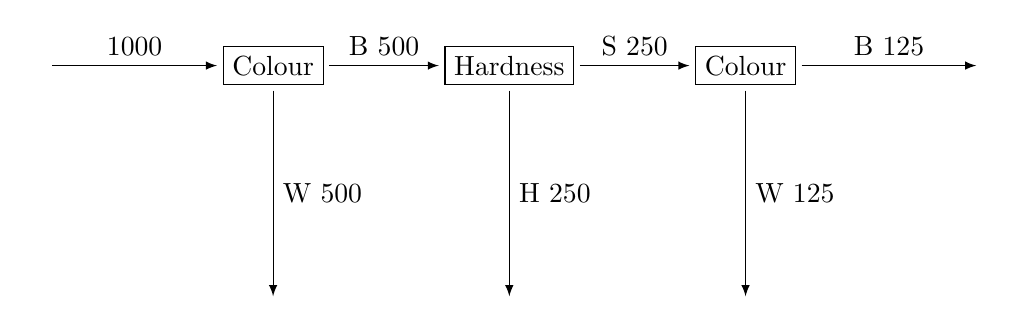
\begin{tikzpicture}[shorten >=4pt,node distance=3cm,on grid,auto]
        \node[draw,rectangle] (a)   {Colour};
        \node[] (a_left) [left=of a] {};
        \coordinate[below of=a] (a_below);
        \node[draw,rectangle] (b) [right=of a] {Hardness};
        \coordinate[below of=b] (b_below);
        \node[draw,rectangle] (c) [right=of b] {Colour};
        \coordinate[right of=c] (c_right);
        \coordinate[below of=c] (c_below);
        \path[-latex,shorten >= 2pt, shorten <= 2pt]
            (a_left)
                edge node {$1000$} (a)
            (a)
                edge node {B $500$} (b)
                edge node {W $500$} (a_below)
            (b)
                edge node {S $250$} (c)
                edge node {H $250$} (b_below)
            (c)
                edge node {B $125$} (c_right)
                edge node {W $125$} (c_below);
    \end{tikzpicture}
    \caption{Repeated detectors that detect colour and hardness, demonstrating the uncertainty principle. By measuring the hardness, we became uncertain of the colour.}
    \label{fig:experiment1}
\end{figure}

% \subsection{Sub Section 1}
% \label{sub_sec:sub_section_1}

% \begin{theorem}
% This is a theorem.
% \end{theorem}
% \begin{proof}
% This is a proof.
% \end{proof}
% \begin{example}
% This is an example.
% \end{example}
% \begin{explanation}
% This is an explanation.
% \end{explanation}
% \begin{claim}
% This is a claim.
% \end{claim}
% \begin{corollary}
% This is a corollary.
% \end{corollary}
% \begin{prop}
% This is a proposition.
% \end{prop}
% \begin{lemma}
% This is a lemma.
% \end{lemma}
% \begin{question}
% This is a question.
% \end{question}
% \begin{solution}
% This is a solution.
% \end{solution}
% \begin{exercise}
% This is an exercise.
% \end{exercise}
% \begin{definition}[Definition]
% This is a definition.
% \end{definition}
% \begin{note}
% This is a note.
% \end{note}

% subsection sub_section_1 (end)

\newpage
  
\lesson{Oct 19 2022 Wen (12:28:10)}{Lecture Title}

\subsection{Sub Section 2}
\label{sub_sec:sub_section_2}

\begin{theorem}
This is a theorem.
\end{theorem}
\begin{proof}
This is a proof.
\end{proof}
\begin{example}
This is an example.
\end{example}
\begin{explanation}
This is an explanation.
\end{explanation}
\begin{claim}
This is a claim.
\end{claim}
\begin{corollary}
This is a corollary.
\end{corollary}
\begin{prop}
This is a proposition.
\end{prop}
\begin{lemma}
This is a lemma.
\end{lemma}
\begin{question}
This is a question.
\end{question}
\begin{solution}
This is a solution.
\end{solution}
\begin{exercise}
This is an exercise.
\end{exercise}
\begin{definition}[Definition]
This is a definition.
\end{definition}
\begin{note}
This is a note.
\end{note}

% subsection sub_section_2 (end)

\newpage
  \lesson{Thu, 2 February 2023, 2:50pm -- 4:10pm}{Week 2, Thursday}

`The state of a quantum system corresponds to a vector in a vector space of complex numbers.'

\begin{definition}
  A \emph{vector} is a list of numbers.
  The length (or magnitude; denoted by $\lvert\ket{v}\rvert$) of a vector can be found by calculating the square root of the sum of squares of the horizontal and vertical components.
  Scalar multiplication can be performed by multiplying every value of a vector by the scalar. A \emph{unit vector} is a vector, $\vec{v}$ with a magnitude $\lvert v \rvert = 1$.
  Vector addition can be performed by adding every element in a vector with the element in the corresponding position in another vector.
  Vector multiplication (also referred to as finding a dot product, or an inner product; denoted by the product $\braket{v}{w}$) can be done between two vectors with the same dimensions. If the result of the multiplication is $0$, the two vectors are \emph{orthogonal}.
\end{definition}
\begin{example}
  Row (`bra' in Dirac notation): $\bra{v} = \begin{bmatrix}
    2 & 3 & 4
  \end{bmatrix}$\\
  Column (`ket' in Dirac notation): $\ket{w} = 
  \begin{bmatrix}
    2\\
    3\\
    4
  \end{bmatrix}
  $\\
  Magnitude: $\ket{v} = 
  \begin{bmatrix}
    a\\
    b\\
  \end{bmatrix}$\\
  $\lvert\ket{w}\rvert = \sqrt{a^2 + b^2}$\\
  Scalar multiplication: $\ket{v} = 
  \begin{bmatrix}
    3\\
    -2
  \end{bmatrix}$\\
  $4 \cdot \ket{v} = 4 \cdot
  \begin{bmatrix}
    3\\
    -2
  \end{bmatrix} = \begin{bmatrix}
    12\\
    -8
  \end{bmatrix}$\\
  Vector addition: $\begin{bmatrix}
    1\\
    2\\
    3
  \end{bmatrix} + \begin{bmatrix}
    7\\
    -3\\
    4
  \end{bmatrix} = \begin{bmatrix}
    8\\
    -1\\
    7
  \end{bmatrix}$\\
  Multiplication: $\begin{bmatrix}
    2 & 3 & 4
  \end{bmatrix} \cdot \begin{bmatrix}
    -1\\
    2\\
    7
  \end{bmatrix} = -2 + 6 + 28 = 32$\\
\end{example}

\begin{note}
  For the purposes of this course, we must be able to find the length of a vector, preform scalar multiplication, perform vector addition, and check for orthogonality.
\end{note}

\begin{definition}
  A set of \emph{basis vectors} is a set of vectors that can be combined in a linear combination to make any other vector in the vector space.
\end{definition}
\begin{example}
  Possible basis vectors with two dimensions:\\
  $\begin{bmatrix}
    76.9513\\
    \pi
  \end{bmatrix} = 76.9513 \cdot \begin{bmatrix}
    1\\
    0
  \end{bmatrix} - \pi \cdot \begin{bmatrix}
    0\\
    1
  \end{bmatrix}$\\
  Possible basis vectors with three dimensions:\\
  $\begin{bmatrix}
    1\\
    0\\
    0
  \end{bmatrix} \begin{bmatrix}
    0\\
    1\\
    0
  \end{bmatrix} \begin{bmatrix}
    0\\
    0\\
    1
  \end{bmatrix}$
\end{example}

\begin{note}
  $\ket{→} = \begin{bmatrix}
    \frac{1}{\sqrt{2}}\\
    -\frac{1}{\sqrt{2}}
  \end{bmatrix}$\\
  $\ket{←} = \begin{bmatrix}
    \frac{1}{\sqrt{2}}\\
    \frac{1}{\sqrt{2}}
  \end{bmatrix}$\\
  $\ket{↗} = \begin{bmatrix}
    \frac{1}{2}\\
    \frac{-\sqrt{3}}{2}
  \end{bmatrix}$\\
  $\ket{↙} = \begin{bmatrix}
    \frac{\sqrt{3}}{2}\\
    \frac{1}{2}
  \end{bmatrix}$
\end{note}

% \subsection{Sub Section 3}
% \label{sub_sec:sub_section_3}

% \begin{theorem}
% This is a theorem.
% \end{theorem}
% \begin{proof}
% This is a proof.
% \end{proof}
% \begin{example}
% This is an example.
% \end{example}
% \begin{explanation}
% This is an explanation.
% \end{explanation}
% \begin{claim}
% This is a claim.
% \end{claim}
% \begin{corollary}
% This is a corollary.
% \end{corollary}
% \begin{prop}
% This is a proposition.
% \end{prop}
% \begin{lemma}
% This is a lemma.
% \end{lemma}
% \begin{question}
% This is a question.
% \end{question}
% \begin{solution}
% This is a solution.
% \end{solution}
% \begin{exercise}
% This is an exercise.
% \end{exercise}
% \begin{definition}[Definition]
% This is a definition.
% \end{definition}
% \begin{note}
% This is a note.
% \end{note}

% subsection sub_section_2 (end)

\newpage
  \lesson{Tue, 7 February 2023, 2:50pm -- 4:10pm}{Week 3, Tuesday}

Qubits are represented by unit vectors.

\begin{definition}
    A vector is \emph{orthonormal} if it is both a unit vector and orthogonal.
\end{definition}

\begin{example}
    The following are the basis vectors for $R^3$:
    $\begin{bmatrix}
        1\\
        0\\
        0
    \end{bmatrix}
    \begin{bmatrix}
        0\\
        1\\
        0
    \end{bmatrix}
    \begin{bmatrix}
        0\\
        0\\
        1
    \end{bmatrix}$

    This means that any vector can be written as a linear combination of these basis vectors.

    If we were talking about spin, for example, we could use $R^2$, with the following basis vectors:\\
    $\ket{\uparrow} = \begin{bmatrix}
        1\\
        0
    \end{bmatrix}\\
    \ket{\downarrow} = \begin{bmatrix}
        0\\
        1
    \end{bmatrix}\\
    \ket{\rightarrow} = \begin{bmatrix}
        \frac{1}{\sqrt{2}}\\
        \frac{1}{\sqrt{2}}
    \end{bmatrix}\\
    \ket{\leftarrow} = \begin{bmatrix}
        \frac{1}{\sqrt{2}}\\
        \frac{1}{\sqrt{2}}
    \end{bmatrix}$

    Meaning,\\
    $
    \ket{\nearrow} = \ket{\uparrow} \cdot \ket{\rightarrow} = \begin{bmatrix}
        \frac{1}{2}\\
        \frac{-\sqrt{3}}{2}
    \end{bmatrix}\\
    \ket{\swarrow} = \ket{\downarrow} \cdot \ket{\leftarrow} \begin{bmatrix}
        \frac{\sqrt{3}}{2}\\
        \frac{1}{2}
    \end{bmatrix}
    $.
\end{example}

\begin{definition}
    A \emph{matrix is a rectangular array of numbers.}\\
    The `gates' that are the primary components of quantum computing algorithms correspond to matricies.
\end{definition}

\begin{definition}
    To \emph{transpose} a matrix means to `rotate' it so that its rows become columns, and its columns become rows.
\end{definition}

\begin{example}
    $M = \begin{bmatrix}
        1 & 4\\
        2 & 5\\
        3 & 6
    \end{bmatrix}$\\
    $M$ has $3$ rows by $2$ columns.

    $M^T = \begin{bmatrix}
        1 & 2 & 3\\
        4 & 5 & 6
    \end{bmatrix}$\\
    $M^T$ has $2$ rows by $3$ columns.
\end{example}

If multiplying two matricies, one with dimensions $n \times m$ and the other with dimensions $m \times p$, then the result will have dimensions $n \times p$ (ie, the resultant matrix's dimensions will be number of the first matrix's rows, by the number of the second matrix's columns).

\begin{example}
    $
    \begin{bmatrix}
        1 & 4\\
        2 & 5\\
        3 & 6
    \end{bmatrix}
    \cdot
    \begin{bmatrix}
        -2 & 1 & 3\\
        4 & 7 & -2
    \end{bmatrix}
    =
    \begin{bmatrix}
        14 & 29 & -5\\
        16 & 37 & -4\\
        18 & 45 & -3
    \end{bmatrix}
    $
\end{example}

\begin{definition}
    An \emph{identity matrix} is a matrix when, multiplied with another matrix, simply yields that other matrix.
\end{definition}

\begin{example}
    $
    \begin{bmatrix}
        14 & 29 & -5\\
        16 & 37 & -4\\
        18 & 45 & -3
    \end{bmatrix}
    \cdot
    \begin{bmatrix}
        1 & 0 & 0\\
        0 & 1 & 0\\
        0 & 0 & 1
    \end{bmatrix}
    =
    \begin{bmatrix}
        14 & 29 & -5\\
        16 & 37 & -4\\
        18 & 45 & -3
    \end{bmatrix}
    $
\end{example}

\begin{note}
    If a matrix, $H$, were multiplied by its transpose (ie, $H \cdot H^T$), and if the multiplication were to yield an identity matrix, $I$, then it is orthogonal. In other words, if $H \cdot H^T = I$, then $H$ is orthogonal. When dealing with complex numbers, this is called a \emph{unitary matrix} instead, rather than an `orthogonal matrix'.
\end{note}

\begin{definition}
    A \emph{tensor product} (represented as $A \otimes B$) can be found by, for each value in the left-hand side, multiplying said value with all of the values on the right-hand side. This operation can be referred to as calculating the \emph{Kronecker product} or \emph{matrix direct product}, when dealing specifically with matricies as opposed to other tensors.\\
    A \emph{tensor} is a generalisation of matricies; where a matrix has two dimensions (rows and columns), a tensor can have any number of dimensions.
\end{definition}

\begin{example}
    $
    \begin{bmatrix}
        2\\
        3
    \end{bmatrix}
    \otimes
    \begin{bmatrix}
        -1\\
        4\\
        7
    \end{bmatrix}
    =
    \begin{bmatrix}
        -2\\
        8\\
        14\\
        -3\\
        12\\
        21
    \end{bmatrix}
    $
\end{example}

The state of a quantum system corresponds to a vector.
The state of a quantum system is a tensor product of qubits.
A vector is separable if it can be written as a tensor product of two other vecotrs.
A vector is entangled if it \emph{cannot} be written as the tensor product of two other vectors.

% \subsection{Sub Section 3}
% \label{sub_sec:sub_section_3}

% \begin{theorem}
% This is a theorem.
% \end{theorem}
% \begin{proof}
% This is a proof.
% \end{proof}
% \begin{example}
% This is an example.
% \end{example}
% \begin{explanation}
% This is an explanation.
% \end{explanation}
% \begin{claim}
% This is a claim.
% \end{claim}
% \begin{corollary}
% This is a corollary.
% \end{corollary}
% \begin{prop}
% This is a proposition.
% \end{prop}
% \begin{lemma}
% This is a lemma.
% \end{lemma}
% \begin{question}
% This is a question.
% \end{question}
% \begin{solution}
% This is a solution.
% \end{solution}
% \begin{exercise}
% This is an exercise.
% \end{exercise}
% \begin{definition}[Definition]
% This is a definition.
% \end{definition}
% \begin{note}
% This is a note.
% \end{note}

% subsection sub_section_2 (end)

\newpage
  \lesson{Tue, 7 February 2023, 2:50pm -- 4:10pm}{Week 3, Tuesday}

`The state of a quantum system is a vector in a vector space of complex numbers.'

Using the following basis vectors, $\ket{↑} = \ket{0} = \begin{bmatrix}
    1\\
    0
\end{bmatrix}$, $\ket{↓} = \ket{1} = \begin{bmatrix}
    0\\
    1
\end{bmatrix}$, a quantum state can be represented as $a\ket{0} + b\ket{1}$, where $a$ and $b$ are probability amplitudes (ie, $a^2$ is the probability of getting $\ket{0}$, $b^2$ is the probability of getting $\ket{1}$, and $a^2 + b^2 = 1$). To determine if a quantum state is valid, square the values of $a$ and $b$, and then add them together; if the sum of the squares is not equal to $1$, then the state is invalid.

If we `measure' a qubit in the horizontal direction we are using the basis vectors $(\begin{bmatrix}
    \frac{1}{\sqrt{2}}\\
    -\frac{1}{\sqrt{2}}
\end{bmatrix}, \begin{bmatrix}
    \frac{1}{\sqrt{2}}\\
    \frac{1}{\sqrt{2}}
\end{bmatrix})$.
Some of the values that we're going to repeatedly run into may be familiar from an earlier education in trigonometry.\\
$\sin(45\degree) = \frac{1}{\sqrt{2}}\\
\cos(45\degree) = \frac{1}{\sqrt{2}}\\
\sin(30\degree) = \frac{1}{2} \qquad \cos(60\degree) = \frac{1}{2}\\
\cos(30\degree) = \frac{\sqrt{3}}{2} \qquad \sin(60\degree) = \frac{\sqrt{3}}{2}$\\

\begin{note}
    We cannot distinguish between $\ket{v}$ and $-\ket{v}$.\\
    $\ket{v} = a\ket{0} + b\ket{1}$ has the same probabilities involved as $-\ket{v} = -a\ket{0} - b\ket{1}$ (being $a^2$ for $\ket{0}$ and $b^2$ for $\ket{1}$).
\end{note}

If we were to rotate our observation appparatus (or perspective) by $\Theta\degree$, the new basis vectors would be $(\begin{bmatrix}
    \cos(\Theta)\\
    -\sin(\Theta)
\end{bmatrix}, \begin{bmatrix}
    \sin(\Theta)\\
    \cos(\Theta)
\end{bmatrix})$.

% \subsection{Sub Section 3}
% \label{sub_sec:sub_section_3}

% \begin{theorem}
% This is a theorem.
% \end{theorem}
% \begin{proof}
% This is a proof.
% \end{proof}
% \begin{example}
% This is an example.
% \end{example}
% \begin{explanation}
% This is an explanation.
% \end{explanation}
% \begin{claim}
% This is a claim.
% \end{claim}
% \begin{corollary}
% This is a corollary.
% \end{corollary}
% \begin{prop}
% This is a proposition.
% \end{prop}
% \begin{lemma}
% This is a lemma.
% \end{lemma}
% \begin{question}
% This is a question.
% \end{question}
% \begin{solution}
% This is a solution.
% \end{solution}
% \begin{exercise}
% This is an exercise.
% \end{exercise}
% \begin{definition}[Definition]
% This is a definition.
% \end{definition}
% \begin{note}
% This is a note.
% \end{note}

% subsection sub_section_2 (end)

\newpage
  \lesson{Tue, 14 February 2023, 2:50pm -- 4:10pm}{Week 4, Tuesday}

\begin{definition}
    A \emph{qubit} is a unit vector (`ket') in $C^2$.\
    When we measure a qubit, we are, in effect, choosing a direction for measurement. Which actually means that we are choosing an orthonormal basis vector.
\end{definition}

\begin{note}
    To represent classical bits, we can do so with the equation, $\ket{v} = x \cdot \ket{b_1} + y \cdot \ket{b_2}$ where $x^2 + y^2 = 1$.\\
    We will always write it so that $\ket{b_1} = 0$ and that $\ket{b_2} = 1$, not the other way around; the order in which we write our basis vectors conveys that the first will represent a $0$, and that the second will represent a $1$.
\end{note}

\begin{figure}[h]
    \centering
    \begin{adjustbox}{width=\textwidth}
    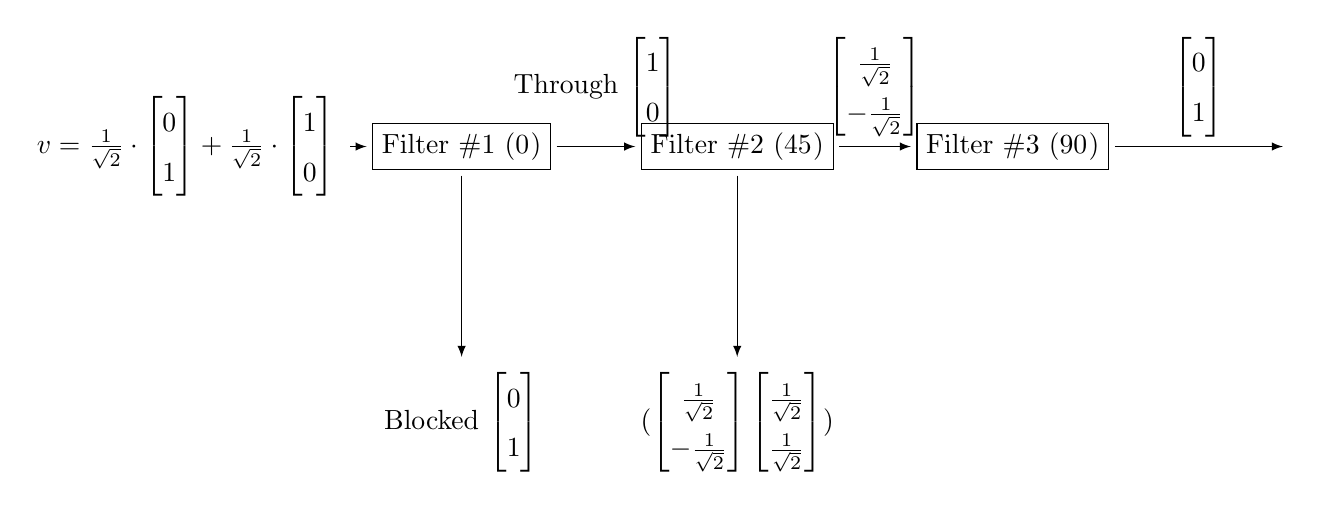
\begin{tikzpicture}[shorten >=1pt,node distance=3.5cm,on grid,auto]
        \node[draw,rectangle] (a)   {Filter \#1 ($0^{\degree}$)};
        \node[] (a_left) [left=of a] {$\ket{v} = \frac{1}{\sqrt{2}}\cdot\begin{bmatrix}0\\1\end{bmatrix} + \frac{1}{\sqrt{2}}\cdot\begin{bmatrix}1\\0\end{bmatrix}$};
        \node[below of=a] (a_below) {Blocked $\begin{bmatrix}0\\1\end{bmatrix}$};

        \node[draw,rectangle,right of=a] (b)   {Filter \#2 ($45^{\degree})$};
        \node[below of=b] (b_below) {$(\begin{bmatrix}\frac{1}{\sqrt{2}}\\-\frac{1}{\sqrt{2}}\end{bmatrix} \begin{bmatrix}\frac{1}{\sqrt{2}}\\\frac{1}{\sqrt{2}}\end{bmatrix})$};
        
        \node[draw,rectangle,right of=b] (c)   {Filter \#3 ($90^{\degree})$};
        \coordinate[right of=c] (c_right);
        \path[-latex,shorten >= 2pt, shorten <= 2pt]
            (a_left)
                edge node {} (a)
            (a)
                edge node {} (a_below)
                edge node {Through $\begin{bmatrix}1\\0\end{bmatrix}$} (b)           
            (b)
                edge node {} (b_below)
                edge node {$\begin{bmatrix}\frac{1}{\sqrt{2}}\\-\frac{1}{\sqrt{2}}\end{bmatrix}$} (c)
            (c)
                edge node {$\begin{bmatrix}0\\1\end{bmatrix}$} (c_right);
    \end{tikzpicture}
    \end{adjustbox}
    \caption{Three repeated filters, blocking photons. The probabilities became a certain outcome.}\label{fig:experiment4}
\end{figure}

\newpage

\begin{definition}
    When two waves collide and destroy one another, that is \emph{destructive interference}. When the two waves combine, that is \emph{constructive interference}.
\end{definition}

\begin{example}
    Find $a$ and $b$ when $\ket{v} = a \cdot \begin{bmatrix}
        1\\
        0
    \end{bmatrix} + b \cdot \begin{bmatrix}
        0\\
        1
    \end{bmatrix}$, where $\ket{v}$ is the interaction between $\ket{←}$ and $\ket{→}$.\\
    $\ket{v} = \frac{1}{\sqrt{2}} \cdot \ket{←} + \frac{1}{\sqrt{2}} \cdot \ket{→} = \frac{1}{\sqrt{2}} \cdot \begin{bmatrix}\frac{1}{\sqrt{2}}\\\frac{1}{\sqrt{2}}\end{bmatrix} + \frac{1}{\sqrt{2}} \cdot \begin{bmatrix}\frac{1}{\sqrt{2}}\\-\frac{1}{\sqrt{2}}\end{bmatrix} = \begin{bmatrix}\frac{1}{2}\\\frac{1}{2}\end{bmatrix} + \begin{bmatrix}\frac{1}{2}\\-\frac{1}{2}\end{bmatrix} = \begin{bmatrix}1\\0\end{bmatrix}$.\\
    Therefore, $a = 1$, $b = 0$. $\ket{←}$ and $\ket{→}$, both with their own probabilities, constructively interfered to achieve one certain outcome.
\end{example}


% \subsection{Sub Section 3}
% \label{sub_sec:sub_section_3}

% \begin{theorem}
% This is a theorem.
% \end{theorem}
% \begin{proof}
% This is a proof.
% \end{proof}
% \begin{example}
% This is an example.
% \end{example}
% \begin{explanation}
% This is an explanation.
% \end{explanation}
% \begin{claim}
% This is a claim.
% \end{claim}
% \begin{corollary}
% This is a corollary.
% \end{corollary}
% \begin{prop}
% This is a proposition.
% \end{prop}
% \begin{lemma}
% This is a lemma.
% \end{lemma}
% \begin{question}
% This is a question.
% \end{question}
% \begin{solution}
% This is a solution.
% \end{solution}
% \begin{exercise}
% This is an exercise.
% \end{exercise}
% \begin{definition}[Definition]
% This is a definition.
% \end{definition}
% \begin{note}
% This is a note.
% \end{note}

% subsection sub_section_2 (end)

\newpage
  \lesson{Thu, 23 February 2023, 2:50pm -- 4:10pm}{Week 5, Thursday}

\begin{note}
    A system of $n$ qubits will be in $C^{2^n}$ space; ie, if you preform tensor multiplication on $n$ qubits (each being in $C^2$ space--meaning each vector has two elements), you will get $C^{2^n}$ space--meaning the resultant vector will have $2^n$ elements.
\end{note}

\begin{note}
    If two qubits are \emph{not} entangled, then we can examine each one independently. Additionally, we can represent this state both as a vector in $C^4$ space, and as the tensor product of two vectors in $C^2$ space.
\end{note}

Suppose we wanted to perform tensor multiplication with groupings; to do so, we would multiply as we would any other algebraic expression: $\ket{vw} = (a \ket{0} + b \ket{1}) \otimes (c \ket{0} + d \ket{1}) = (ac \ket{00} + ad \ket{01} + bc \ket{10} + bd \ket{11})$, where $\ket{0} = \begin{bmatrix}
    1\\
    0
\end{bmatrix}$ and $\ket{1} = \begin{bmatrix}
    0\\
    1
\end{bmatrix}$.

\begin{note}
    $\ket{v} \otimes \ket{w} = \ket{v} \ket{w} = \ket{vw} \neq \braket{v}{w}$.
\end{note}

The standard basis vectors for $C^4 = C^2 \otimes C^2$ space are $\ket{00}$, $\ket{01}$, $\ket{10}$, and $\ket{11}$. This is equivalent to $\begin{bmatrix}
    1\\
    0\\
    0\\
    0
\end{bmatrix}$, $\begin{bmatrix}
    0\\
    1\\
    0\\
    0
\end{bmatrix}$, $\begin{bmatrix}
    0\\
    0\\
    1\\
    0
\end{bmatrix}$, and $\begin{bmatrix}
    0\\
    0\\
    0\\
    1
\end{bmatrix}$.

% \subsection{Sub Section 3}
% \label{sub_sec:sub_section_3}

% \begin{theorem}
% This is a theorem.
% \end{theorem}
% \begin{proof}
% This is a proof.
% \end{proof}
% \begin{example}
% This is an example.
% \end{example}
% \begin{explanation}
% This is an explanation.
% \end{explanation}
% \begin{claim}
% This is a claim.
% \end{claim}
% \begin{corollary}
% This is a corollary.
% \end{corollary}
% \begin{prop}
% This is a proposition.
% \end{prop}
% \begin{lemma}
% This is a lemma.
% \end{lemma}
% \begin{question}
% This is a question.
% \end{question}
% \begin{solution}
% This is a solution.
% \end{solution}
% \begin{exercise}
% This is an exercise.
% \end{exercise}
% \begin{definition}[Definition]
% This is a definition.
% \end{definition}
% \begin{note}
% This is a note.
% \end{note}

% subsection sub_section_2 (end)

\newpage
  \lesson{Tue, 28 February 2023, 2:50pm – 4:10pm}{Week 6, Tuesday}

Two qubits are entangled if, when we measure (observe) one, the state of the other qubit changes instantaneously. The state of any quantum system corresponds to a unit vector in a vector space; that vector can be represented as a linear combination of basis vectors. If two qubits are \emph{not} entangled, then we can examine (measure) one qubit without affecting the state of the other---they are independent. Suppose that the basis vectors that we are using for the first qubit are $\ket{a_1}$ and $\ket{a_2}$, and the basis vectors that we are using for the second qubit are $\ket{b_1}$ and $\ket{b_2}$. Then the state of this system of two qubits is represented by a vector in $R^2$ like $r\ket{a_0 b_0} + s\ket{a_0 b_1} + t\ket{a_1 b_0} + u\ket{a_1 b_1}$. Since $r$, $s$, $t$, and $u$ are probability amplitudes, $r^2 + s^2 + t^2 + u^2 = 1$.

\begin{example}
    \textbf{Separable (not entangled; unentangled)}
    
    $\ket{v} = x_0\ket{a_0} + x_1\ket{a_1} \qquad x_0^2 +x_1^2 = 1$

    $\ket{w} = y_0\ket{b_0} + y_1\ket{b_1} \qquad y_0^2 +y_1^2 = 1$\\

    $\ket{v} \otimes \ket{w} = (x_0\ket{a_0} + x_1\ket{a_1}) \otimes (y_0\ket{b_0} + y_1\ket{b_1}) = x_0y_0\ket{a_0 b_0} + x_0y_1\ket{a_0 b_1} + x_1y_0\ket{a_1 b_0} + x_1y_1\ket{a_1 b_1}$\\

    The squared probability amplitudes sum up to $1$.\\
    $(x_0 y_0)^2 + (x_0 y_1)^2 + (x_1 y_0)^2 + (x_1 y_1)^2 = 1$\\
    To demonstrate this we can use the fact that $x_0^2 + x_1^2 = 1$ and $y_0^2 + y_1^2 = 1$.\\
    $x_0^2(y_0^2 + y_1^2) + x_1^2(y_0^2 + y_1^2) = 1$\\
    $x_0^2 + x_1^2 = 1$
\end{example}

If a vector is entangled, then it cannot be represented as the tensor product of two vectors, $\begin{bmatrix}
    a\\
    b
\end{bmatrix} \otimes \begin{bmatrix}
    c\\
    d
\end{bmatrix} = \begin{bmatrix}
    ac\\
    ad\\
    bc\\
    bd
\end{bmatrix}$.\\
A quick trick to determine if a vector in $C^4$ is entangled is to check if the product of the first and last elements is equal to the product of the middle two elements; if it is, then the vector is not entangled---it is separable. If the products are different, then the vector is entangled (ie, if $ac \cdot bd \neq ad \cdot bc$, then the vector is entangled).

\pagebreak

\begin{example}
    \textbf{Separable (not entangled; unentangled)}

    $(a\ket{0} + b\ket{1}) \otimes (c\ket{0} + d\ket{1}) = ac\ket{0 0} + ad\ket{0 1} + bc\ket{1 0} + bd\ket{1 1}$
    \begin{enumerate}
        \item What is the probability that the second qubit is $\ket{0}$?
        \item Now, let's measure the first qubit. Suppose we get $\ket{0}$. What is the probability that the second qubit is $\ket{0}$?
        \item Now what is the probability that the second qubit is $\ket{0}$?
    \end{enumerate}
    \textbf{\emph{Solution}}
    \begin{enumerate}
        \item $P(\ket{0}) = (ac)^2 + (bc)^2 = a^2 c^2 + b^2 c^2 = c^2(a^2 + b^2) = c^2$.
        \item  $ac\ket{00} + ad\ket{01}$. This is an invalid quantum state; $(ac)^2 + (ad)^2 \neq 1$. We know this because we know that $(ac)^2 + (ad)^2 + (bc)^2 + (bd)^2 = 1$. We can normalise using the length, $\sqrt{(ac)^2 + (ad)^2} = \sqrt{a^2 c^2 + a^2 d^2} = \sqrt{a^2(c^2 + d^2)} = a$. $\frac{ac\ket{00}}{a} + \frac{ad\ket{01}}{a} = c\ket{00} + d\ket{01}$. This is a valid quantum state.
        \item $P(\ket{0}) = (c)^2 = c^2$. This is the same as the probability that the second qubit is $\ket{0}$ when we don't measure the first qubit. This means that the first qubit and the second qubit are independent. They are \emph{not} entangled.
    \end{enumerate}
\end{example}

\begin{example}
    \textbf{Entangled}

    $a\ket{00} + b\ket{01} + c\ket{10} + d\ket{11}$\\
    \begin{enumerate}
        \item What is the probability that the second qubit is $\ket{0}$?
        \item Now, let's measure the first qubit. Suppose we get $\ket{0}$. What is the probability that the second qubit is $\ket{0}$?
        \item Now, what is the probability that the second qubit is $\ket{0}$?
    \end{enumerate}
    \textbf{\emph{Solution}}
    \begin{enumerate}
        \item $a^2 + c^2$
        \item The system state becomes $a\ket{00} + b\ket{10}$. This is not a valid quantum state, because $(a)^2 + (b)^2 + (c)^2 + (d)^2 = 1$. We can normalise using the length, $\sqrt{a^2 + b^2}$. $\frac{a\ket{00}}{\sqrt{a^2 + b^2}} + \frac{b\ket{10}}{\sqrt{a^2 + b^2}}$. This is a valid quantum state.
        \item $\frac{a^2}{a^2 + b^2}$. This does not equal $a^2 + c^2$ (the probability that the second qubit is $\ket{0}$ when we don't measure the first qubit). This means that the first qubit and the second qubit are not independent. They are entangled; they both changed.
    \end{enumerate}
\end{example}

Hadamard gate: $\mathrm{H} = \frac{1}{\sqrt{2}}\begin{bmatrix}
    1 & 1\\
    1 & -1
\end{bmatrix} = \begin{bmatrix}
    \frac{1}{\sqrt{2}} & \frac{1}{\sqrt{2}}\\
    \frac{1}{\sqrt{2}} & -\frac{1}{\sqrt{2}}
\end{bmatrix}$.

CNot gate: $\mathrm{CNot} = \begin{bmatrix}
    1 & 0 & 0 & 0\\
    0 & 1 & 0 & 0\\
    0 & 0 & 0 & 1\\
    0 & 0 & 1 & 0
\end{bmatrix} \begin{bmatrix}
    a\\
    b\\
    c\\
    d
\end{bmatrix} = \begin{bmatrix}
    a\\
    b\\
    d\\
    c
\end{bmatrix}$.

% \subsection{Sub Section 3}
% \label{sub_sec:sub_section_3}

% \begin{theorem}
% This is a theorem.
% \end{theorem}
% \begin{proof}
% This is a proof.
% \end{proof}
% \begin{example}
% This is an example.
% \end{example}
% \begin{explanation}
% This is an explanation.
% \end{explanation}
% \begin{claim}
% This is a claim.
% \end{claim}
% \begin{corollary}
% This is a corollary.
% \end{corollary}
% \begin{prop}
% This is a proposition.
% \end{prop}
% \begin{lemma}
% This is a lemma.
% \end{lemma}
% \begin{question}
% This is a question.
% \end{question}
% \begin{solution}
% This is a solution.
% \end{solution}
% \begin{exercise}
% This is an exercise.
% \end{exercise}
% \begin{definition}[Definition]
% This is a definition.
% \end{definition}
% \begin{note}
% This is a note.
% \end{note}

% subsection sub_section_2 (end)

\newpage
  \lesson{Thu, 2 March 2023, 2:50pm -- 4:10pm}{Week 6, Thursday}

\begin{definition}
    The \emph{Copenhagen interpretation}, put simply, is that the wave function is a description of the state of the universe, and that the universe is in a superposition of states; in other words, everything is existing in all possible states at once. It's a broad term describing the interpretation of quantum mechanics shared by Niels Bohr and Werner Heisenberg---the term comes from the work that both performed together at the University of Copenhagen.
\end{definition}

\begin{definition}
    The \emph{EPR Paradox} is a thought experiment that was first proposed by Albert Einstein, Boris Podolsky, and Nathan Rosen in 1935. The paper describing the paradox argued that quantum mechanics was `incomplete', and that it was impossible to reconcile the theory with special relativity. The paradox is based on the idea that two particles, $A$ and $B$, are entangled, and that the measurement of the spin of particle $A$ will instantaneously affect the spin of particle $B$. This is a violation of the principle of locality, which states that the speed of light is the fastest possible speed of information transfer.
\end{definition}

\begin{definition}
    The \emph{Bell Inequality} is a mathematical inequality that was first proposed by John Stewart Bell in 1964. The inequality is a response to the EPR Paradox, and it describes an experiment that, if performed, would show whether or not the Copenhagen interpretation is correct or not.
    
    % $\frac{1}{\sqrt{2}} \ket{00} + \frac{1}{\sqrt{2}} \ket{11} = \frac{1}{\sqrt{2}}(\ket{0} \otimes \ket{0}) + \frac{1}{\sqrt{2}}(\ket{1} \otimes \ket{1}) = \frac{1}{\sqrt{2}} (\begin{bmatrix}
    %     1\\
    %     0
    % \end{bmatrix} \otimes \begin{bmatrix}
    %     1\\
    %     0
    % \end{bmatrix}) + \frac{1}{\sqrt{2}}(\begin{bmatrix}
    %     0\\
    %     1
    % \end{bmatrix} \otimes \begin{bmatrix}
    %     0\\
    %     1
    % \end{bmatrix}) = \frac{1}{\sqrt{2}} \begin{bmatrix}
    %     1\\
    %     0\\
    %     0\\
    %     0
    % \end{bmatrix} + \frac{1}{\sqrt{2}} \begin{bmatrix}
    %     0\\
    %     0\\
    %     0\\
    %     1
    % \end{bmatrix} = \frac{1}{\sqrt{2}} \begin{bmatrix}
    %     1\\
    %     0\\
    %     0\\
    %     1
    % \end{bmatrix} = \begin{bmatrix}
    %     \frac{1}{\sqrt{2}}\\
    %     0\\
    %     0\\
    %     \frac{1}{\sqrt{2}}
    % \end{bmatrix}$.\\

    Bell suggests performing the following experiment:
    \begin{enumerate}
        \item Create a stream of pairs of entangled particles.
        \item Measure and record the spin of one particle in each pair, using one randomly chosen direction out of three, $0^{\degree}$, $120^{\degree}$, $240^{\degree}$ ($\ket{\uparrow}$, $\ket{\downarrow}$, $\ket{\searrow}$, $\ket{\nwarrow}$, $\ket{\swarrow}$, $\ket{\nearrow}$)---the answer will be either $0$ or $1$.
        \item Measure the spin of the other particle in each pair, randomly choosing the direction again for the remaining particles.
        \item When all the pairs are measured, there will be two strings of $0$s and $1$s, one for each particle in each pair. If the pairs are the same in both strings (ie, if they `agree'), note that the outcome was $A$ in a new, third string---and if they are different (ie, if they `disagree'), note that the outcome was $D$.
        \item In the long run, the pairs will be the same (ie, the outcome will be $A$) about $\frac{1}{2}$ of the time, and different (ie, the outcome will be $D$) about $\frac{1}{2}$ of the time. Knowing that $P(A) = \frac{1}{2}$ and that $P(D) = \frac{1}{2}$, we know that the third, final string will be half $A$s and half $D$s.
    \end{enumerate}

    The sample space of this experiment would resemble the following:\\

    \begin{adjustbox}{width=\textwidth}
        \begin{tabular}{lll}
        $0^{\degree}$ & $120^{\degree}$ & $240^{\degree}$ \\
        $0$ & $0$ & $0$ \\
        $0$ & $0$ & $1$ \\
        $0$ & $1$ & $0$ \\
        $0$ & $1$ & $1$ \\
        $1$ & $0$ & $0$ \\
        $1$ & $0$ & $1$ \\
        $1$ & $1$ & $0$ \\
        $1$ & $1$ & $1$ \\
        \end{tabular}
        \begin{tabular}{|l|l|l|l|l|l|l|l|l|l|}
        \hline ($0^{\degree}$, $0^{\degree}$) & ($0^{\degree}$, $120^{\degree}$) & ($0^{\degree}$, $240^{\degree}$) & ($120^{\degree}$, $0^{\degree}$) & ($120^{\degree}$, $120^{\degree}$) & ($120^{\degree}$, $240^{\degree}$) & ($240^{\degree}$, $0^{\degree}$) & ($240^{\degree}$, $120^{\degree}$) & ($240^{\degree}$, $240^{\degree}$) & Number of $A$s \\
        \hline $A$ & $A$ & $A$ & $A$ & $A$ & $A$ & $A$ & $A$ & $A$ & $9$ \\
        \hline $A$ & $A$ & $D$ & $A$ & $A$ & $D$ & $D$ & $D$ & $A$ & $5$ \\
        \hline $A$ & $D$ & $A$ & $D$ & $A$ & $D$ & $A$ & $D$ & $A$ & $5$ \\
        \hline $A$ & $D$ & $D$ & $D$ & $A$ & $A$ & $D$ & $A$ & $A$ & $5$ \\
        \hline $A$ & $D$ & $D$ & $D$ & $A$ & $A$ & $D$ & $A$ & $A$ & $5$ \\
        \hline $A$ & $D$ & $A$ & $D$ & $A$ & $D$ & $A$ & $D$ & $A$ & $5$ \\
        \hline $A$ & $A$ & $D$ & $A$ & $A$ & $D$ & $D$ & $D$ & $A$ & $5$ \\
        \hline $A$ & $A$ & $A$ & $A$ & $A$ & $A$ & $A$ & $A$ & $A$ & $9$ \\
        \hline
        \end{tabular}
    \end{adjustbox}\\

    The sample space demonstrates, however, that the smallest possible proportion of $A$s is $\frac{5}{9}$. When performing the experiment in reality, the proportion of $A$s and $D$s will be closer to $\frac{1}{2}$ than $\frac{5}{9}$, validating the Copenhagen interpretation.
\end{definition}

% \subsection{Sub Section 3}
% \label{sub_sec:sub_section_3}

% \begin{theorem}
% This is a theorem.
% \end{theorem}
% \begin{proof}
% This is a proof.
% \end{proof}
% \begin{example}
% This is an example.
% \end{example}
% \begin{explanation}
% This is an explanation.
% \end{explanation}
% \begin{claim}
% This is a claim.
% \end{claim}
% \begin{corollary}
% This is a corollary.
% \end{corollary}
% \begin{prop}
% This is a proposition.
% \end{prop}
% \begin{lemma}
% This is a lemma.
% \end{lemma}
% \begin{question}
% This is a question.
% \end{question}
% \begin{solution}
% This is a solution.
% \end{solution}
% \begin{exercise}
% This is an exercise.
% \end{exercise}
% \begin{definition}[Definition]
% This is a definition.
% \end{definition}
% \begin{note}
% This is a note.
% \end{note}

% subsection sub_section_2 (end)

\newpage
  \lesson{Thu, 9 March 2023, 2:50pm -- 4:10pm}{Week 7, Thursday}

All quantum operations (except measurements) are reversible and are represented by unitary matrices.

\begin{definition}
    An operation is \emph{reversible} if, from the output, we can determine the inputs.
\end{definition}

\begin{definition}
    A \emph{unitary matrix} is a matrix whose inverse is its \emph{conjugate} transpose. An \emph{orthogonal matrix} is a matrix whose inverse is its transpose. See \textbf{Definition 4.12} and \textbf{Definition 4.13} from \textbf{Lecture 4}.
\end{definition}

The behaviour of the CNOT gate can be represented with the following two tables:\\
\begin{tabular}{l|l}
    Input & Output\\
    \hline
    $x \ y$ & $x \ x \oplus y$\\
    $0 \ 0$ & $0 \ 0$\\
    $0 \ 1$ & $0 \ 1$\\
    $1 \ 0$ & $1 \ 1$\\
    $1 \ 1$ & $1 \ 0$
\end{tabular}
\begin{tabular}{l|l}
    Input & Output\\
    \hline
    $\ket{00}$ & $\ket{00}$\\
    $\ket{01}$ & $\ket{01}$\\
    $\ket{10}$ & $\ket{11}$\\
    $\ket{11}$ & $\ket{10}$
\end{tabular}\\

CNOT:\\
$\begin{bmatrix}
    1 & 0 & 0 & 0\\
    0 & 1 & 0 & 0\\
    0 & 0 & 0 & 1\\
    0 & 0 & 1 & 0
\end{bmatrix} \begin{bmatrix}
    a\\
    b\\
    c\\
    d
\end{bmatrix} = \begin{bmatrix}
    a\\
    b\\
    d\\
    c
\end{bmatrix}$

\begin{example}
    $\mathrm{CNOT}(r\ket{00} + s\ket{01} + t\ket{10} + u\ket{11}) = r\ket{00} + s\ket{01} + u\ket{10} + t\ket{11}$. The probabilitiy amplitudes for $\ket{10}$ and $\ket{11}$ are flipped.
\end{example}

\pagebreak

\begin{explanation}
    CNOT is a unitary matrix:\\
    $\begin{bmatrix}
        1 & 0 & 0 & 0\\
        0 & 1 & 0 & 0\\
        0 & 0 & 0 & 1\\
        0 & 0 & 1 & 0
    \end{bmatrix} \begin{bmatrix}
        1 & 0 & 0 & 0\\
        0 & 1 & 0 & 0\\
        0 & 0 & 0 & 1\\
        0 & 0 & 1 & 0
    \end{bmatrix} = \begin{bmatrix}
        1 & 0 & 0 & 0\\
        0 & 1 & 0 & 0\\
        0 & 0 & 1 & 0\\
        0 & 0 & 0 & 1
    \end{bmatrix}$\\
    It is its own inverse and its own conjugate transpose.
\end{explanation}

\begin{figure}[h]
    \centering
    \begin{tikzpicture}[shorten >=1pt,node distance=3.5cm,on grid,auto]
        \node[] (start_top) {$\frac{1}{\sqrt{2}}\ket{0} + \frac{1}{\sqrt{2}}\ket{1}$};
        \node[right of=start_top,circle,draw=black,fill=black] (end_top) {};
        \coordinate[right of=end_top] (beyond_top);
        \node[below of=start_top] (start_bottom) {$\ket{0}$};
        \node[right of=start_bottom] (end_bottom) {$\oplus$};
        \coordinate[right of=end_bottom] (beyond_bottom);
        
        \path[-,shorten >= 2pt, shorten <= 2pt]
            (start_top)
                edge node {} (end_top)
            (end_top)
                edge node {} (end_bottom)
                edge node {} (beyond_top)
            (start_bottom)
                edge node {} (end_bottom)
            (end_bottom)
                edge node {} (beyond_bottom);
    \end{tikzpicture}
    \caption{$(\frac{1}{\sqrt{2}}\ket{0} + \frac{1}{\sqrt{2}}\ket{1}) \otimes \ket{0} = \frac{1}{\sqrt{2}}\ket{00} + \frac{1}{\sqrt{2}}\ket{10} = \frac{1}{\sqrt{2}}\begin{bmatrix}
        1\\
        0\\
        0\\
        0
    \end{bmatrix} \begin{bmatrix}
        0\\
        0\\
        1\\
        0
    \end{bmatrix} = \frac{1}{\sqrt{2}}\begin{bmatrix}
        1\\
        0\\
        1\\
        0
    \end{bmatrix}$}\label{fig:lec10fig1}
\end{figure}

$\frac{1}{\sqrt{2}}\begin{bmatrix}
    1\\
    0\\
    0\\
    1
\end{bmatrix} = \frac{1}{\sqrt{2}}\begin{bmatrix}
    1\\
    0\\
    0\\
    0
\end{bmatrix} + \frac{1}{\sqrt{2}}\begin{bmatrix}
    0\\
    0\\
    0\\
    1
\end{bmatrix} = \frac{1}{\sqrt{2}}\ket{00} + \frac{1}{\sqrt{2}}\ket{11}$.

Quantum gates with one input:
\begin{enumerate}
    \item Pauli's gate
    \item Identity gate ($\begin{bmatrix}
        1 & 0\\
        0 & 1
    \end{bmatrix}$)
    \item Z gate ($\begin{bmatrix}
        1 & 0\\
        0 & -1
    \end{bmatrix}$; relative phase shift)
    \item X gate ($\begin{bmatrix}
        0 & 1\\
        1 & 0
    \end{bmatrix}$; flips the probability amplitudes)
    \item Y gate ($\begin{bmatrix}
        0 & -i\\
        i & 0
    \end{bmatrix}$)
    \item Hadamard gate ($\frac{1}{\sqrt{2}}\begin{bmatrix}
        1 & 1\\
        1 & -1
    \end{bmatrix}$)
\end{enumerate}
All of the above gates are reversible, are equal to their own transpose (except for the Y gate), and yield the identity gate when multiplied by their transpose.

\begin{example}
    $\mathrm{z}(a\ket{0} + b\ket{1}) = a\ket{0} - b\ket{1}$
\end{example}

\begin{note}
    In the above example, we are observing a \emph{relative phase shift}.
\end{note}

\pagebreak

\begin{figure}[ht]
    \centering
    \begin{tikzpicture}[shorten >=1pt,node distance=3.5cm,on grid,auto]
        \node[] (start_top) {$\ket{0}$};
        \node[right of=start_top,draw] (h) {$H$};
        \node[right of=h,circle,draw=black,fill=black] (end_top) {};
        \coordinate[right of=end_top] (beyond_top);
        \node[below of=start_top] (start_bottom) {$\ket{0}$};
        \node[below of=end_top] (end_bottom) {$\oplus$};
        \coordinate[right of=end_bottom] (beyond_bottom);
        
        \path[-]
            (start_top)
                edge node {} (h)
            (h)
                edge node {$\frac{1}{\sqrt{2}}\ket{0} + \frac{1}{\sqrt{2}}\ket{1}$} (end_top)
            (end_top)
                edge node {} (end_bottom)
                edge node {} (beyond_top)
            (start_bottom)
                edge node {} (end_bottom)
            (end_bottom)
                edge node {} (beyond_bottom);
    \end{tikzpicture}
    \caption{An example of Bell's Circuit, with an input of $\ket{00}$.}\label{fig:lec10fig2}
\end{figure}

At the start of the circuit, the state of the system is $\ket{0} \otimes \ket{0} = \ket{00}$. After passing through the Hadamard gate, the state of the system is $(\frac{1}{\sqrt{2}} \ket{0} + \frac{1}{\sqrt{2}} \ket{1}) \otimes \ket{0} = \frac{1}{\sqrt{2}}\ket{00} + \frac{1}{\sqrt{2}} \ket{10} = \frac{1}{\sqrt{2}} \begin{bmatrix}
    1\\
    0\\
    0\\
    0\\
\end{bmatrix} + \frac{1}{\sqrt{2}} \begin{bmatrix}
    0\\
    0\\
    1\\
    0
\end{bmatrix} = \frac{1}{\sqrt{2}} \begin{bmatrix}
    1\\
    0\\
    1\\
    0
\end{bmatrix}$. Lastly, after passing through the CNOT gate, the state of the system is $\frac{1}{\sqrt{2}} \begin{bmatrix}
    1\\
    0\\
    0\\
    1
\end{bmatrix} = \frac{1}{\sqrt{2}}\begin{bmatrix}
    1\\
    0\\
    0\\
    0\\
\end{bmatrix} + \frac{1}{\sqrt{2}} \begin{bmatrix}
    0\\
    0\\
    0\\
    1
\end{bmatrix} = \frac{1}{\sqrt{2}} \ket{00} + \frac{1}{\sqrt{2}} \ket{11} = \mathrm{B}(\ket{00})$, which is an entangled state.\\

There is a pattern to Bell's Circuit:\\
$\mathrm{B}(\ket{00}) = \frac{1}{\sqrt{2}} \ket{00} + \frac{1}{\sqrt{2}} \ket{11}$\\
$\mathrm{B}(\ket{01}) = \frac{1}{\sqrt{2}} \ket{01} + \frac{1}{\sqrt{2}} \ket{10}$\\
$\mathrm{B}(\ket{10}) = \frac{1}{\sqrt{2}} \ket{00} - \frac{1}{\sqrt{2}} \ket{11}$\\
$\mathrm{B}(\ket{11}) = \frac{1}{\sqrt{2}} \ket{01} - \frac{1}{\sqrt{2}} \ket{10}$\\

\begin{question}
    What are the standard basis vectors for $R^4$?
\end{question}

\hfill

\begin{solution}
    $\begin{bmatrix}
        1\\
        0\\
        0\\
        0
    \end{bmatrix}$
    $\begin{bmatrix}
        0\\
        1\\
        0\\
        0
    \end{bmatrix}$
    $\begin{bmatrix}
        0\\
        0\\
        1\\
        0
    \end{bmatrix}$
    $\begin{bmatrix}
        0\\
        0\\
        0\\
        1
    \end{bmatrix}$\\
    $\ket{00}$, $\ket{01}$, $\ket{10}$, $\ket{11}$
\end{solution}

If one were to pass an input through Bell's Circuit, and then to the reverse Bell's Circuit, the output would be the same as the input.

% \subsection{Sub Section 3}
% \label{sub_sec:sub_section_3}

% \begin{theorem}
% This is a theorem.
% \end{theorem}
% \begin{proof}
% This is a proof.
% \end{proof}
% \begin{example}
% This is an example.
% \end{example}
% \begin{explanation}
% This is an explanation.
% \end{explanation}
% \begin{claim}
% This is a claim.
% \end{claim}
% \begin{corollary}
% This is a corollary.
% \end{corollary}
% \begin{prop}
% This is a proposition.
% \end{prop}
% \begin{lemma}
% This is a lemma.
% \end{lemma}
% \begin{question}
% This is a question.
% \end{question}
% \begin{solution}
% This is a solution.
% \end{solution}
% \begin{exercise}
% This is an exercise.
% \end{exercise}
% \begin{definition}[Definition]
% This is a definition.
% \end{definition}
% \begin{note}
% This is a note.
% \end{note}

% subsection sub_section_2 (end)

\newpage
  \lesson{Tue, 14 March 2023, 2:50pm -- 4:10pm}{Week 8, Tuesday}

\begin{definition}
    The \emph{no cloning theorem} states that it is not possible to \underline{copy} an arbitrary quantum state without destroying the original. In other words, it is possible to `cut and paste', but it is not possible to `copy and paste'. To develop an intuitive understanding of why this is, suppose we have a qubit in a superposition, $a \ket{0} + b \ket{1}$, and we wished to copy it---if we wished to measure the qubit to copy it, the superposition collapses.
\end{definition}

Suppose we had a gate to copy a qubit, $G$.
If we were to supply it an input to copy and a qubit to copy the first qubit onto, we would observe the following outputs:\\
$G(\ket{00}) = \ket{00}$\\
$G(\ket{10}) = \ket{11}$\\
$G(\frac{1}{\sqrt{2}} \ket{0} + \frac{1}{\sqrt{2}} \ket{1} \otimes \ket{0}) = (\frac{1}{\sqrt{2}} \ket{0} + \frac{1}{\sqrt{2}} \ket{1}) \otimes (\frac{1}{\sqrt{2}} \ket{0} + \frac{1}{\sqrt{2}} \ket{1})$\\
$G(\frac{1}{\sqrt{2}} \ket{00} + \frac{1}{\sqrt{2}} \ket{10}) = \frac{1}{\sqrt{2}} \ket{00} + \frac{1}{\sqrt{2}} \ket{01} + \frac{1}{\sqrt{2}} \ket{10} + \frac{1}{\sqrt{2}} \ket{11}$\\
$G(\frac{1}{\sqrt{2}} \ket{00} + \frac{1}{\sqrt{2}} \ket{10}) = G(\frac{1}{\sqrt{2}}\ket{00}) + G(\frac{1}{\sqrt{2}}\ket{10}) = \frac{1}{\sqrt{2}} G(\ket{00}) + \frac{1}{\sqrt{2}} G(\ket{10}) = \frac{1}{\sqrt{2}} \ket{00} + \frac{1}{\sqrt{2}} \ket{11}$\\
As you can see, the last two outputs are not the same, despite the same input; this is a contradiction. The contradiction demonstrates that such a gate cannot exist.
\begin{figure}[ht]
    \centering
    \begin{tikzpicture}[shorten >=1pt,node distance=3.5cm,on grid,auto]
        \node[] (start_top) {$\ket{0}$};
        \node[right of=start_top,draw] (h) {$H$};
        \node[right of=h,circle,draw=black,fill=black] (end_top) {};
        \coordinate[right of=end_top] (beyond_top);
        \node[below of=start_top] (start_bottom) {$\ket{0}$};
        \node[below of=end_top] (end_bottom) {$\oplus$};
        \coordinate[right of=end_bottom] (beyond_bottom);
        
        \path[-]
            (start_top)
                edge node {\textcolor{DarkGreen}{$\ket{00} = \ket{0} \otimes \ket{0}$}} (h)
            (h)
                edge node {$\frac{1}{\sqrt{2}}\ket{0} + \frac{1}{\sqrt{2}}\ket{1}$} (end_top)
                edge node[below] {\textcolor{DarkGreen}{\begin{adjustbox}{width=3cm}$(\frac{1}{\sqrt{2}}\ket{0} + \frac{1}{\sqrt{2}}\ket{1}) \otimes \ket{0} = \frac{1}{\sqrt{2}} \ket{00} + \frac{1}{\sqrt{2}} \ket{10} = \frac{1}{\sqrt{2}} \begin{bmatrix}
                    1\\
                    0\\
                    1\\
                    0
                \end{bmatrix}$\end{adjustbox}}} (end_top)
            (end_top)
                edge node {} (end_bottom)
                edge node {\begin{adjustbox}{width=3cm}$\frac{1}{\sqrt{2}}\ket{00} + \frac{1}{\sqrt{2}}\ket{11} = \frac{1}{\sqrt{2}}\begin{bmatrix}
                    1\\
                    0\\
                    0\\
                    1
                \end{bmatrix}$\end{adjustbox}} (beyond_top)
            (start_bottom)
                edge node {} (end_bottom)
            (end_bottom)
                edge node {\textcolor{DarkGreen}{\begin{adjustbox}{width=3.5cm}$\frac{1}{\sqrt{2}}\begin{bmatrix}
                    1\\
                    0\\
                    0\\
                    1
                \end{bmatrix} = \frac{1}{\sqrt{2}}\ket{00} + \frac{1}{\sqrt{2}}\ket{11} = \frac{1}{\sqrt{2}}\begin{bmatrix}
                    1\\
                    0\\
                    0\\
                    0
                \end{bmatrix} + \frac{1}{\sqrt{2}}\begin{bmatrix}
                    0\\
                    0\\
                    0\\
                    1
                \end{bmatrix}$\end{adjustbox}}} (beyond_bottom);
    \end{tikzpicture}
    \caption{An example of Bell's Circuit, with an input of $\ket{00}$. When you have a circuit of unentangled qubits, qubits on parallel lines are represented by a tensor product.}\label{fig:lec11fig1}
\end{figure}

`Sequential gates are represented by the product of matrices'.

The `C' in `C-NOT' stands for `controlled'---it is a `controlled operation'.\\
The `NOT' gate:\\
$\begin{bmatrix}
    0 & 1\\
    1 & 0
\end{bmatrix}$.\\
\begin{claim}
    The `C-NOT' gate acts analagously to an \verb+if+ statement. If the first qubit is $1$, then apply the `NOT' gate to the second qubit. In other words, if the $1^{\underline{\text{st}}}$ qubit is $0$, the second qubit remains the same and the second qubit is flipped.
\end{claim}

\begin{example}
    Suppose we had a hypothetical gate which looked like:\\
    $\begin{bmatrix}
        a & b\\
        c & d
    \end{bmatrix}$. Let's say we wished to create a `controlled' version of this gate, called $A$:\\
    $A = \begin{bmatrix}
        1 & 0 & 0 & 0\\
        0 & 1 & 0 & 0\\
        0 & 0 & a & b\\
        0 & 0 & c & d
    \end{bmatrix}$.\\
    $A(\ket{00}) = \ket{00}$, $A(\ket{01}) = \ket{01}$, $A(\ket{10}) = \ket{1} \otimes \begin{bmatrix}
        a\\
        c
    \end{bmatrix}$, $A(\ket{11}) = \ket{1} \otimes \begin{bmatrix}
        b\\
        d
    \end{bmatrix}$.\\
\end{example}

The `Taffoli' gate has two controls bits and one output:
\[ \begin{bmatrix}
    1 & 0 & 0 & 0 & 0 & 0 & 0 & 0\\
    0 & 1 & 0 & 0 & 0 & 0 & 0 & 0\\
    0 & 0 & 1 & 0 & 0 & 0 & 0 & 0\\
    0 & 0 & 0 & 1 & 0 & 0 & 0 & 0\\
    0 & 0 & 0 & 0 & 1 & 0 & 0 & 0\\
    0 & 0 & 0 & 0 & 0 & 1 & 0 & 0\\
    0 & 0 & 0 & 0 & 0 & 0 & 0 & 1\\
    0 & 0 & 0 & 0 & 0 & 0 & 1 & 0
\end{bmatrix} \]
We can think of this gate as the `C-C-NOT' gate (a `controlled'-`controlled'-`NOT' gate). It is reversible, and universal in the context of classical computing (just like `NAND').\\

\pagebreak

\begin{figure}[ht]
    \centering
    \begin{tikzpicture}[shorten >=1pt,node distance=3.5cm,on grid,auto]
        \node[] (start_top) {$\ket{x}$};
        \node[right of=start_top,circle,draw=black,fill=black] (end_top) {};
        \coordinate[right of=end_top] (beyond_top);

        \node[below of=start_top] (start_middle) {$\ket{y}$};
        \node[below of=end_top,circle,draw=black,fill=black] (end_middle) {};
        \coordinate[right of=end_middle] (beyond_middle);
        
        \node[below of=start_middle] (start_bottom) {$\ket{z}$};
        \node[below of=end_middle] (end_bottom) {$\oplus$};
        \coordinate[right of=end_bottom] (beyond_bottom);
        
        \path[-]
            (start_top)
                edge node {} (end_top)
            (end_top)
                edge node {} (end_bottom)
                edge node {$\ket{x}$} (beyond_top)
            (start_middle)
                edge node {} (end_middle)
            (end_middle)
                edge node {$\ket{y}$} (beyond_middle)
            (start_bottom)
                edge node {} (end_bottom)
            (end_bottom)
                edge node {$\ket{z \oplus (x \wedge y)}$} (beyond_bottom);
    \end{tikzpicture}
    \caption{A circuit demonstrating the Taffoli gate.}\label{fig:lec11fig2}
\end{figure}

\begin{note}
    There is a relationship between the two sides of the exclusive `or' operation ($\oplus$):\\
    $0 \oplus 0 = 0$, $0 \oplus 1 = 1$, $0 \oplus x = x$.\\
    $1 \oplus 0 = 1$, $1 \oplus 1 = 0$, $1 \oplus x = \overline{x}$.
\end{note}

\begin{question}
    Are there any quantum gates that are universal?
\end{question}

\hfill

\begin{solution}
    No.
\end{solution}

\begin{question}
    How many 1-qubit quantum gates are there?
\end{question}

\hfill

\begin{solution}
    Infinity.
\end{solution}

The `Fredkin' gate has one control bit, two outputs:
\[ \begin{bmatrix}
    1 & 0 & 0 & 0 & 0 & 0 & 0 & 0\\
    0 & 1 & 0 & 0 & 0 & 0 & 0 & 0\\
    0 & 0 & 1 & 0 & 0 & 0 & 0 & 0\\
    0 & 0 & 0 & 1 & 0 & 0 & 0 & 0\\
    0 & 0 & 0 & 0 & 1 & 0 & 0 & 0\\
    0 & 0 & 0 & 0 & 0 & 0 & 1 & 0\\
    0 & 0 & 0 & 0 & 0 & 1 & 0 & 0\\
    0 & 0 & 0 & 0 & 0 & 0 & 0 & 1
\end{bmatrix} \]
If $\ket{x} = 0$, $\ket{y}$ and $\ket{z}$ are unchanged. If $\ket{x} = \ket{1}$, $\ket{y^{\prime}}$ = $\ket{z}$, $\ket{z^{\prime}} = \ket{y}$.

\begin{figure}[ht]
    \centering
    \begin{tikzpicture}[shorten >=1pt,node distance=3.5cm,on grid,auto]
        \node[] (start_top) {$\ket{x}$};
        \node[right of=start_top,circle,draw=black,fill=black] (end_top) {};
        \coordinate[right of=end_top] (beyond_top);

        \node[below of=start_top] (start_middle) {$\ket{y}$};
        \node[below of=end_top,cross out,draw=black] (end_middle) {};
        \coordinate[right of=end_middle] (beyond_middle);
        
        \node[below of=start_middle] (start_bottom) {$\ket{z}$};
        \node[below of=end_middle,cross out,draw=black] (end_bottom) {};
        \coordinate[right of=end_bottom] (beyond_bottom);
        
        \path[-]
            (start_top)
                edge node {} (end_top)
            (end_top)
                edge node {} (end_middle)
                edge node {$\ket{x}$} (beyond_top)
            (start_middle)
                edge node {} (end_middle)
            (end_middle)
                edge node {} (end_bottom)
                edge node {$\ket{y^{\prime}}$} (beyond_middle)
            (start_bottom)
                edge node {} (end_bottom)
            (end_bottom)
                edge node {$\ket{z^{\prime}}$} (beyond_bottom);
    \end{tikzpicture}
    \caption{A circuit demonstrating the Fredkin gate.}\label{fig:lec11fig3}
\end{figure}

% \subsection{Sub Section 3}
% \label{sub_sec:sub_section_3}

% \begin{theorem}
% This is a theorem.
% \end{theorem}
% \begin{proof}
% This is a proof.
% \end{proof}
% \begin{example}
% This is an example.
% \end{example}
% \begin{explanation}
% This is an explanation.
% \end{explanation}
% \begin{claim}
% This is a claim.
% \end{claim}
% \begin{corollary}
% This is a corollary.
% \end{corollary}
% \begin{prop}
% This is a proposition.
% \end{prop}
% \begin{lemma}
% This is a lemma.
% \end{lemma}
% \begin{question}
% This is a question.
% \end{question}
% \begin{solution}
% This is a solution.
% \end{solution}
% \begin{exercise}
% This is an exercise.
% \end{exercise}
% \begin{definition}[Definition]
% This is a definition.
% \end{definition}
% \begin{note}
% This is a note.
% \end{note}

% subsection sub_section_2 (end)

\newpage
  \lesson{Thu, 16 March 2023, 2:50pm -- 4:10pm}{Week 8, Thursday}

As a reminder, the Pauli-X gate (`NOT' gate) is $X = \begin{bmatrix}
    0 & 1 \\
    1 & 0\\
\end{bmatrix}$, the Pauli-Y gate is $Y = i \begin{bmatrix}
    0 & -1 \\
    1 & 0\\
\end{bmatrix}$, and the Pauli-Z gate is $Z = \begin{bmatrix}
    1 & 0 \\
    0 & -1\\
\end{bmatrix}$.

The Pauli gates perform the following operations on the basis states:\\
\begin{itemize}
    \item $X(a \ket{0} + b \ket{1}) = b \ket{0} + a \ket{1}$
    \item $Y(a \ket{0} + b \ket{1}) = b \ket{0} - a \ket{1}$
    \item $Z(a \ket{0} + b \ket{1}) = a \ket{0} - b \ket{1}$
\end{itemize}

If one were to pass the following inputs into Bell's Circuit ($B$), these would be the outputs:
\begin{itemize}
    \item $B(\ket{00}) = \frac{1}{\sqrt{2}} \ket{00} + \frac{1}{\sqrt{2}} \ket{11}$
    \item $B(\ket{01}) = \frac{1}{\sqrt{2}} \ket{01} + \frac{1}{\sqrt{2}} \ket{10}$
    \item $B(\ket{10}) = \frac{1}{\sqrt{2}} \ket{00} - \frac{1}{\sqrt{2}} \ket{11}$
    \item $B(\ket{11}) = \frac{1}{\sqrt{2}} \ket{01} - \frac{1}{\sqrt{2}} \ket{10}$
\end{itemize}

\begin{definition}
    \emph{Quantum communication} is the exploitation of entanglement to transmit information.
\end{definition}
\subsection{Quantum Communication Protocols}
\label{sub_sec:quantum_communication_protocols}
\begin{itemize}
    \item Superdense coding
        \begin{itemize}
            \item To communicate a number of classical bits by use of a smaller number of qubits. In other words, using one qubit to send two classical bits.
            \item Start with two entangled qubits in superposition, one sent to Alice, and the other sent to Bob.
            \item Alice wants to send two classical bits to Bob; she can send either $00$, $01$, $10$, or $11$---essentially, she is going to send Bob one qubit.
            \item If she wants to send $00$, she does nothing (she applies the identity gate, $I$). The quantum state is unchanged, being $\frac{1}{\sqrt{2}} \ket{00} + \frac{1}{\sqrt{2}} \ket{11}$.
            \item If she wants to send $01$, she applies the Pauli-X (or `NOT') gate, $X$. The quantum state is now $\frac{1}{\sqrt{2}} \ket{10} + \frac{1}{\sqrt{2}} \ket{01}$.
            \item If she wants to send $10$, she applies the Pauli-Z gate, $Z$. The quantum state is now $\frac{1}{\sqrt{2}} \ket{00} - \frac{1}{\sqrt{2}} \ket{11}$.
            \item If she wants to send $11$, she applies the Pauli-Y gate, $Y$. The quantum state is now $\frac{1}{\sqrt{2}} \ket{01} - \frac{1}{\sqrt{2}} \ket{10}$.
            \item The quantum states that result from Alice's transformations match our expected outputs of Bell's circuit. Knowing this, Bob now applies the reverse Bell circuit, $B^{\dagger}$, to the qubit he received from Alice. This will give him the two classical bits he wanted to receive.
        \end{itemize}
    \item Quantum teleportation
        \begin{itemize}
            \item Sending two classical bits to transmit (`teleport') one qubit.
            \item Bob and Alice share an entangled pair, and Alice has another qubit of her own in some state, $a \ket{0} + b \ket{1}$. She wants to send Bob her qubit, but she cannot clone it, so she must `cut-and-paste' it (she will lose it, but Bob will have it).
            \item Alice entangles her two qubits, entangling all three qubits. She first applies the Hadamard gate, with the quantum state becoming $(a \ket{0} + b \ket{1}) \otimes (\frac{1}{\sqrt{2}} \ket{00} + \frac{1}{\sqrt{2}} \ket{11}) = \frac{a}{\sqrt{2}} \ket{000} + \frac{a}{\sqrt{2}} \ket{011} + \frac{b}{\sqrt{2}} \ket{100} + \frac{b}{\sqrt{2}} \ket{111} = \frac{a}{\sqrt{2}} \ket{00} \otimes \ket{0} + \frac{a}{\sqrt{2}} \ket{01} \otimes \ket{1} + \frac{b}{\sqrt{2}} \ket{10} \otimes \ket{0} + \frac{b}{\sqrt{2}} \ket{11} \otimes \ket{1}$. After applying the CNOT gate to her qubits, the state becomes $\frac{a}{\sqrt{2}} \ket{00} \otimes \ket{0} + \frac{a}{\sqrt{2}} \ket{01} \otimes \ket{1} + \frac{b}{\sqrt{2}} \ket{11} \otimes \ket{0} + \frac{b}{\sqrt{2}} \ket{10} \otimes \ket{11} = \frac{a}{\sqrt{2}} \ket{0} \otimes \ket{0} \otimes \ket{0} + \frac{a}{\sqrt{2}} \ket{0} \otimes \ket{1} \otimes \ket{1} + \frac{b}{\sqrt{2}} \ket{1} \otimes \ket{1} \otimes \ket{0} + \frac{b}{\sqrt{2}} \ket{1} \otimes \ket{0} \otimes \ket{11}$. The state of the qubit Alice wants to send to Bob is now entangled with the two qubits she shared with Bob.
            \item She then applies the Hadamard gate to the qubit which she wants to send, and the state becomes $\frac{a}{\sqrt{2}}(\frac{1}{\sqrt{2}} \ket{0} + \frac{1}{\sqrt{2}} \ket{1}) \otimes \ket{0} \otimes \ket{0} + \frac{a}{\sqrt{2}}(\frac{1}{\sqrt{2}} \ket{0} + \frac{1}{\sqrt{2}} \ket{1}) \otimes \ket{1} \otimes \ket{1} + \frac{b}{\sqrt{2}} (\frac{1}{\sqrt{2}} \ket{0} - \frac{1}{\sqrt{2}} \ket{1}) \otimes \ket{1} \otimes \ket{0} + \frac{b}{\sqrt{2}}(\frac{1}{\sqrt{2}} \ket{0} - \frac{1}{\sqrt{2}} \ket{1}) \otimes \ket{0} \otimes \ket{1} = \frac{1}{2} \ket{00} \otimes (a \ket{0} + b\ket{1}) + \frac{1}{2} \ket{01} \otimes (a \ket{1} + b \ket{0}) + \frac{1}{2} \ket{10} \otimes (a \ket{0} - b \ket{1}) + \frac{1}{2} \ket{11} \otimes (a \ket{1} - b \ket{0})$.
            \item If Alice measures $\ket{00}$, Bob's state is $a \ket{0} + b \ket{1}$. If Alice measures $\ket{01}$, Bob's state is $a \ket{1} + b \ket{0}$. If Alice measures $\ket{10}$, Bob's state is $a \ket{0} - b \ket{1}$. If Alice measures $\ket{11}$, Bob's state is $a \ket{1} - b \ket{1}$.
            \item Alice now sends Bob the two classical bits she measured (ie, sends $00$ if $\ket{00}$, $10$ if $\ket{10}$, etc). If Bob gets $00$, he does nothing (he applies the identity gate, $I$); his state is $a \ket{0} + b\ket{1}$. If Bob gets $01$, he applies the Pauli-X gate, $X$; his state is $a \ket{0} + b \ket{1}$. If Bob gets $10$, he applies the Pauli-Z gate, $Z$. If Bob gets $11$, he applies the Pauli-Y gate, $Y$.
        \end{itemize}
\end{itemize}
% subsection quantum_communication_protocols (end)

% \subsection{Sub Section 3}
% \label{sub_sec:sub_section_3}

% \begin{theorem}
% This is a theorem.
% \end{theorem}
% \begin{proof}
% This is a proof.
% \end{proof}
% \begin{example}
% This is an example.
% \end{example}
% \begin{explanation}
% This is an explanation.
% \end{explanation}
% \begin{claim}
% This is a claim.
% \end{claim}
% \begin{corollary}
% This is a corollary.
% \end{corollary}
% \begin{prop}
% This is a proposition.
% \end{prop}
% \begin{lemma}
% This is a lemma.
% \end{lemma}
% \begin{question}
% This is a question.
% \end{question}
% \begin{solution}
% This is a solution.
% \end{solution}
% \begin{exercise}
% This is an exercise.
% \end{exercise}
% \begin{definition}[Definition]
% This is a definition.
% \end{definition}
% \begin{note}
% This is a note.
% \end{note}

% subsection sub_section_2 (end)

\newpage
  \lesson{Thu, 6 April 2023, 2:50pm -- 4:10pm}{Week 11, Thursday}

\begin{definition}
    \emph{Quantum parallelism} refers to the speedup that we experience with quantum algorithms, as opposed to classical algorithms, which results from the fact that we put our input into a superposition. A quantum algorithm is designed to manipulate these superpositions to get useful results.
\end{definition}

\begin{definition}
    $P$ is the set of problems for which there is a classical algorithm that can solve it in polynomial time.
    $NP$ is the set of problems that can be verified by a classical algorithm in polynomial time.
\end{definition}

The typical steps in a quantum algorithm are as follows:
\begin{enumerate}
    \item Begin with qubits in a particular classical state
    \item Put the system into a superposition of many states
    \item Act on the superposition with several quantum gates
\end{enumerate}

\begin{definition}
    \emph{Deutsch's algorithm} attempts to minimise the query complexity when faced with the following problem:\\

    Given a function $f: \{0, 1\} \rightarrow \{0, 1\}$, is this function constant or balanced?\\
    
    Possible functions could be:
    \begin{itemize}
        \item Constant - 0 ($f(0)=0$, $f(1)=0$)
        \item Constant - 1 ($f(0)=1$, $f(1)=1$)
        \item Identity ($f(0)=0$, $f(1)=1$)
        \item Swap ($f(0)=1$, $f(1)=0$)
    \end{itemize}

    Instead of requiring both $f(0)$ and $f(1)$ to determine the nature of $f$, Deutsch's algorithm requires only one.\\
    The input to the algorithm is the function, $f$. The algorithm represents the possible $f$ functions with quantum gates:

    Constant - 0:\\
    $\begin{bmatrix}
        1 & 1\\
        0 & 0
    \end{bmatrix} \cdot \ket{0} = \ket{0}$\\

    $\begin{bmatrix}
        1 & 1\\
        0 & 0
    \end{bmatrix} \cdot \ket{1} = \ket{0}$\\


    Constant - 1:\\
    $\begin{bmatrix}
        0 & 0\\
        1 & 1
    \end{bmatrix} \cdot \ket{0} = \ket{1}$\\

    $\begin{bmatrix}
        0 & 0\\
        1 & 1
    \end{bmatrix} \cdot \ket{1} = \ket{1}$\\


    Identity:\\
    $\begin{bmatrix}
        1 & 0\\
        0 & 1
    \end{bmatrix} \cdot \ket{0} = \ket{0}$\\

    $\begin{bmatrix}
        1 & 0\\
        0 & 1
    \end{bmatrix} \cdot \ket{1} = \ket{1}$\\


    Swap:\\
    $\begin{bmatrix}
        0 & 1\\
        1 & 0
    \end{bmatrix} \cdot \ket{0} = \ket{1}$\\

    $\begin{bmatrix}
        0 & 1\\
        1 & 0
    \end{bmatrix} \cdot \ket{1} = \ket{0}$\\        
\end{definition}

\begin{figure}[ht]
    \centering
    \begin{quantikz}
        \lstick{$\ket{0}$\\$x$}\slice{A} & \gate{H}\slice{B} & \gate[wires=2]{F}\slice{C} & \gate{H}\slice{D} & \meter{} & \qw \\
        \lstick{$\ket{1}$\\$y$} & \gate{H} & \qw & \qw & \qw & \qw
    \end{quantikz}
    \caption{The circuit for Deutsch's algorithm, where $F(\ket{xy}) = F(\ket{x}, \ket{y}) = \ket{x} \otimes (\ket{y} \oplus f(\ket{x}))$; $F$ is the controlled version of the quantum gate representation of the function, $f$, whichever of the four functions it may be. The state of the system at A is $\ket{01}$, $\frac{1}{2}(\ket{00}-\ket{01}+\ket{10}-\ket{11})$ at B, $\frac{1}{2}(\ket{0} \otimes f(0) - \ket{0} \otimes \overline{f(0)} + \ket{1} \otimes f(1) - \ket{1} \otimes \overline{f(1)})$ at C, and either $\ket{0}$ or $\ket{1}$ at D.}\label{fig:lec13fig1}
\end{figure}

\pagebreak

% \subsection{Sub Section 3}
% \label{sub_sec:sub_section_3}

% \begin{theorem}
% This is a theorem.
% \end{theorem}
% \begin{proof}
% This is a proof.
% \end{proof}
% \begin{example}
% This is an example.
% \end{example}
% \begin{explanation}
% This is an explanation.
% \end{explanation}
% \begin{claim}
% This is a claim.
% \end{claim}
% \begin{corollary}
% This is a corollary.
% \end{corollary}
% \begin{prop}
% This is a proposition.
% \end{prop}
% \begin{lemma}
% This is a lemma.
% \end{lemma}
% \begin{question}
% This is a question.
% \end{question}
% \begin{solution}
% This is a solution.
% \end{solution}
% \begin{exercise}
% This is an exercise.
% \end{exercise}
% \begin{definition}[Definition]
% This is a definition.
% \end{definition}
% \begin{note}
% This is a note.
% \end{note}

% subsection sub_section_2 (end)

\newpage
  \lesson{Tue, 11 April 2023, 2:50pm -- 4:10pm}{Week 12, Tuesday}

In Figure~\ref{fig:lec13fig1}, we saw that the circuit for Deutsch's algorithm has four `slices', A, B, C, and D. Slice A is fairly straightforward, $\ket{01}$, being the inputs, and slice D is also fairly straightforward, either $\ket{0}$ or $\ket{1}$, being the possible outputs.

The state of the system at B is $\frac{1}{\sqrt{2}} (\ket{0} + \ket{1}) \otimes \frac{1}{\sqrt{2}} (\ket{0} - \ket{1}) = \frac{1}{2} (\ket{00} - \ket{01} + \ket{10} - \ket{11})$. The state of the system at C is $F(\frac{1}{2} (\ket{00} - \ket{01} + \ket{10} - \ket{11})) = \frac{1}{2}(F(\ket{00}) - F(\ket{01}) + F(\ket{10}) - F(\ket{11})) = \frac{1}{2}(\ket{0} \otimes (0 \oplus f(0)) - \ket{0} \otimes (1 \oplus f(0))) + (\ket{1} \otimes (0 \oplus f(1)) - \ket{1} \otimes (1 \oplus f(1))) = \frac{1}{2}(\ket{0} \otimes f(0) - \ket{0} \otimes \overline{f(0)} + \ket{1} \otimes f(1) - \ket{1} \otimes \overline{f(1)})$.

The state of the system at C is therefore a superposition of the four possible outputs of the function, $f$:\\

Case 1 ($f(0) = 0$, $f(1) = 0$):\\
$\frac{1}{2}(\ket{00} - \ket{01} + \ket{10} - \ket{11}) = \frac{1}{\sqrt{2}} (\ket{0} + \ket{1}) \otimes \frac{1}{\sqrt{2}} (\ket{0} - \ket{1})$\\

Case 2 ($f(0) = 1$, $f(1) = 1$):\\
$\frac{1}{2}(\ket{01} - \ket{00} + \ket{11} - \ket{10}) = -\frac{1}{2} (\ket{00} - \ket{01} + \ket{10} - \ket{11}) = -\frac{1}{\sqrt{2}} (\ket{0} + \ket{1}) \otimes \frac{1}{\sqrt{2}} (\ket{0} - \ket{1})$\\

Case 3 ($f(0) = 0$, $f(1) = 1$):\\
$\frac{1}{2}(\ket{00} - \ket{01} + \ket{11} - \ket{10}) = \frac{1}{\sqrt{2}} (\ket{0} - \ket{1}) \otimes \frac{1}{\sqrt{2}} (\ket{0} - \ket{1})$\\

Case 4 ($f(0) = 1$, $f(1) = 0$):\\
$\frac{1}{2}(\ket{01} - \ket{00} + \ket{10} - \ket{11}) = -\frac{1}{2} (\ket{00} - \ket{01} + \ket{10} - \ket{11}) = -\frac{1}{\sqrt{2}} (\ket{0} + \ket{1}) \otimes \frac{1}{\sqrt{2}} (\ket{0} - \ket{1})$\\

For Case 1, D can be evaluated as $H(\frac{1}{\sqrt{2}}\ket{0} + \frac{1}{\sqrt{2}}\ket{1}) = \ket{0}$. For Case 2, D can be evaluated as $H(-\frac{1}{\sqrt{2}}\ket{0} + \frac{1}{\sqrt{2}}\ket{1}) = -\ket{0}$. For Case 3, D can be evaluated as $H(\frac{1}{\sqrt{2}}\ket{0} - \frac{1}{\sqrt{2}}\ket{1}) = \ket{1}$. For Case 4, D can be evaluated as $H(-\frac{1}{\sqrt{2}}\ket{0} - \frac{1}{\sqrt{2}}\ket{1}) = -\ket{1}$.

\begin{definition}
    The \emph{Deutsch-Jozsa algorithm} is a quantum algorithm that solves the following problem:\\

    Given a function $f: \{0,1\}^n \rightarrow \{0,1\}$, that is either constant or balanced, determine which it is.\\

    If $n=4$, the problem requires $9$ function calls in the worst case. If $n=3$, the problem requires $5$ function calls in the worst case. If $n=2$, the problem requires $3$ function calls in the worst case. This relationship is modeled by the expression $2^{n-1} + 1$. The Deutsch-Jozsa algorithm requires $1$ function call; it operates in constant time.
\end{definition}

\begin{definition}
    The $H^{\otimes 2}$ gate is $\frac{1}{2} \begin{bmatrix}
        1 & 1 & 1 & 1\\
        1 & -1 & 1 & -1\\
        1 & 1 & -1 & -1\\
        1 & -1 & -1 & 1
    \end{bmatrix} = \frac{1}{\sqrt{2}} \begin{bmatrix}
        H & H\\
        H & -H\\
    \end{bmatrix}$.

    It functions as follows:\\

    $H(\ket{0}) \otimes H(\ket{0}) = \frac{1}{\sqrt{2}} (\ket{0} + \ket{1}) \otimes \frac{1}{\sqrt{2}} (\ket{0} + \ket{1}) = \frac{1}{2} (\ket{00} + \ket{01} + \ket{10} + \ket{11}) = \frac{1}{2} \begin{bmatrix}
        1\\
        1\\
        1\\
        1
    \end{bmatrix}$\\
    
    $H(\ket{0}) \otimes H(\ket{1}) = \frac{1}{2} (\ket{00} - \ket{01} + \ket{10} - \ket{11}) = \frac{1}{2} \begin{bmatrix}
        1\\
        -1\\
        1\\
        -1
    \end{bmatrix}$\\
    
    $H(\ket{1}) \otimes H(\ket{0}) = \frac{1}{\sqrt{2}} (\ket{0} - \ket{1}) \otimes \frac{1}{\sqrt{2}} (\ket{0} + \ket{1}) = \frac{1}{2} (\ket{00} + \ket{01} - \ket{10} - \ket{11}) = \frac{1}{2} \begin{bmatrix}
        1\\
        1\\
        -1\\
        -1
    \end{bmatrix}$\\
    
    $H(\ket{1}) \otimes H(\ket{1}) = \frac{1}{2} (\ket{00} - \ket{10}) \otimes \frac{1}{2}(\ket{0} - \ket{1}) = \frac{1}{2}(\ket{00} - \ket{01} - \ket{10} + \ket{11}) = \frac{1}{2} \begin{bmatrix}
        1\\
        -1\\
        -1\\
        1
    \end{bmatrix}$\\
\end{definition}

\begin{note}
    $H^{\otimes 3} = \frac{1}{\sqrt{2}} \begin{bmatrix}
        H^{\otimes 2} & H^{\otimes 2}\\
        H^{\otimes 2} & -H^{\otimes 2}\\
    \end{bmatrix}$.
\end{note}

\begin{figure}[ht]
    \centering
    \begin{quantikz}
        \lstick{$\ket{00}$\\$x$}\slice{A} & \gate{H^{\otimes 2}}\slice{B} & \gate[wires=2]{F}\slice{C} & \gate{H^{\otimes 2}}\slice{D} & \meter{} & \qw \\
        \lstick{$\ket{1}$\\$y$} & \gate{H} & \qw & \qw & \qw & \qw
    \end{quantikz}
    \caption{The circuit for the Deutsch-Jozsa algorithm when $n = 2$, where $F(x_1, x_2, y) = \ket{x_1 x_2} \otimes (y \oplus f(x_1, x_2))$. At D, the state can be either $\ket{00}$, $\ket{01}$, $\ket{10}$, or $\ket{11}$.}\label{fig:lec14fig1}
\end{figure}

At slice A, the state is $\ket{001}$. At slice B, the state is $\frac{1}{\sqrt{2}} \begin{bmatrix}
    1 & 1 & 1 & 1\\
    1 & -1 & 1 & -1\\
    1 & 1 & -1 & -1\\
    1 & -1 & -1 & 1
\end{bmatrix} \cdot \begin{bmatrix}
    1\\
    0\\
    0\\
    0
\end{bmatrix} = \frac{1}{2} \begin{bmatrix}
    1\\
    1\\
    1\\
    1
\end{bmatrix} = \frac{1}{2} (\ket{00} + \ket{01} + \ket{10} + \ket{11})$. Expressed differently, $\frac{1}{2}(\ket{00} + \ket{01} + \ket{10} + \ket{11}) \otimes \frac{1}{\sqrt{2}} (\ket{0} - \ket{1}) = \frac{1}{2\sqrt{2}} (\ket{000} - \ket{001} + \ket{010} - \ket{011} + \ket{100} - \ket{101} + \ket{110} - \ket{111})$. At slice C, the state is $F(\frac{1}{2\sqrt{2}} (\ket{000} - \ket{001} + \ket{010} - \ket{011} + \ket{100} - \ket{101} + \ket{110} - \ket{111})) = \frac{1}{2\sqrt{2}} (F(\ket{000}) - F(\ket{001}) + F(\ket{010}) - F(\ket{011}) + F(\ket{100}) - F(\ket{101}) + F(\ket{110}) - F(\ket{111})) = \frac{1}{2\sqrt{2}} (\ket{00} \otimes (0 \oplus f(0)) - \ket{00} \otimes (1 \oplus f(00)) + \ket{01} \otimes (0 \oplus f(01)) - \ket{01} \otimes (1 \oplus f(01)) + \ket{10} \otimes (0 \oplus f(10)) - \ket{10} \otimes (1 \oplus f(10)) + \ket{11} \otimes (0 \oplus f(11)) - \ket{11} \otimes (1 \oplus f(11))) = \frac{1}{2\sqrt{2}}(\ket{00} \otimes f(00) - \ket{00} \otimes \overline{f(00)} + \ket{01 \otimes f(01) - \ket{01} \otimes \overline{f(01)} + \ket{01} \otimes f(10)} - \ket{10} \otimes \overline{f(10)} + \ket{11} \otimes f(11) - \ket{11} \otimes \overline{f(11)})$.

\begin{figure}[ht]
    \centering
    \begin{quantikz}
        \lstick{$\ket{0}^n$\\$x$}\slice{A} & \gate{H^{\otimes n}}\slice{B} & \gate[wires=2]{F}\slice{C} & \gate{H^{\otimes n}}\slice{D} & \meter{} & \qw \\
        \lstick{$\ket{1}$\\$y$} & \gate{H} & \qw & \qw & \qw & \qw
    \end{quantikz}
    \caption{The general circuit for the Deutsch-Jozsa algorithm.}\label{fig:lec14fig2}
\end{figure}

% \subsection{Sub Section 3}
% \label{sub_sec:sub_section_3}

% \begin{theorem}
% This is a theorem.
% \end{theorem}
% \begin{proof}
% This is a proof.
% \end{proof}
% \begin{example}
% This is an example.
% \end{example}
% \begin{explanation}
% This is an explanation.
% \end{explanation}
% \begin{claim}
% This is a claim.
% \end{claim}
% \begin{corollary}
% This is a corollary.
% \end{corollary}
% \begin{prop}
% This is a proposition.
% \end{prop}
% \begin{lemma}
% This is a lemma.
% \end{lemma}
% \begin{question}
% This is a question.
% \end{question}
% \begin{solution}
% This is a solution.
% \end{solution}
% \begin{exercise}
% This is an exercise.
% \end{exercise}
% \begin{definition}[Definition]
% This is a definition.
% \end{definition}
% \begin{note}
% This is a note.
% \end{note}

% subsection sub_section_2 (end)

\newpage
  \lesson{Thu, 20 April 2023, 2:50pm -- 4:10pm}{Week 13, Thursday}

\begin{definition}
    \emph{Simon's periodicity algorithm} is a probabilistic algorithm which involves a quantum and a classical part; it solves the following problem:\\

    Given a function $f: \{0, 1\}^n \rightarrow \{0, 1\}^n$ that is periodic, find its period. A period function is $f(x) = f(x \oplus c)$, where $c$ is the period.
\end{definition}

\begin{figure}[ht]
    \centering
    \begin{quantikz}
        \lstick{$\ket{0}^n$\\$x$} & \qw\qwbundle{n} & \gate{H^{\otimes n}} & \qw\qwbundle{n} & \gate[wires=2]{F} & \qw\qwbundle{n} & \gate{H^{\otimes n}} & \qw\qwbundle{n} & \meter{} & \qw \\
        \lstick{$\ket{0}^n$\\$y$} & \qw\qwbundle{n} & \qw & \qw & \qw & \qw\qwbundle{n} & \qw & \qw & \qw & \qw
    \end{quantikz}
    \caption{The general circuit for Simon's periodicity algorithm.}\label{fig:lec15fig1}
\end{figure}

\begin{figure}[ht]
    \centering
    \begin{quantikz}
        \lstick{$\ket{00}$\\$x$}\slice{A} & \qw\qwbundle{2} & \gate{H^{\otimes 2}}\slice{B} & \qw\qwbundle{2} & \gate[wires=2]{F}\slice{C} & \qw\qwbundle{n} & \gate{H^{\otimes 2}}\slice{D} & \qw\qwbundle{2} & \meter{} & \qw \\
        \lstick{$\ket{00}$\\$y$} & \qw\qwbundle{2} & \qw & \qw & \qw & \qw\qwbundle{2} & \qw & \qw & \qw & \qw
    \end{quantikz}
    \caption{The circuit for Simon's periodicity algorithm when $n = 2$, where $F(x_1x_2, y_1y_2) = \ket{x_1x_2} \otimes (y_1y_2 \oplus f(x_1x_2)) = \ket{x_1x_2} \otimes f(x_1x_2)$.}\label{fig:lec15fig2}
\end{figure}

If $\ket{x}$ is an answer that you get from Simon's algorithm, it is \emph{always} true that $x \cdot c = 0$, where $c$ is the period and $x$ is a series of classical bits.\\

Suppose we run the algorithm, when $n = 5$, and we get an answer of $1 0 1 0 0$. This means that $1 \cdot c_0 \oplus 0 \cdot c_1 \oplus 1 \cdot c_2 \oplus 0 \cdot c_3 \oplus 0 \cdot c_4 = 0$, $c_0 \oplus c_2 = 0$, so $c_0 = c_2$. Suppose we run the algorithm again, and get $0 0 1 0 0$; $0 \cdot c_0 \oplus 0 \cdot c_1 \oplus 1 \cdot c_2 \oplus 0 \cdot c_3 \oplus 0 \cdot c_4 = 0 \oplus 0 \oplus c_2 \oplus 0 \oplus 0 = 0$, meaning $c_2 = 0$. If $c_2 = 0$ and $c_0 = c_2$, then $c_0 = 0$. Suppose we run the algorithm a third time, and get $1 1 1 1 0$; $c_0 \oplus c_1 \oplus c_2 \oplus c_3 = 0 = 0 \oplus c_1 \oplus 0 \oplus c_3 = 0 = c_1 \oplus c_3 = 0 = c_1 = 3$. Suppose we run the algorithm a fourth time and get $0 0 1 1 1$; we know that $c_2 \oplus c_3 \oplus c_4 = 0 = c_3 \oplus c_4 = 0$, meaning $c = 0 1 0 1 1$.

\begin{definition}
    \emph{Grover's search algorithm} is an algorithm that solves the following problem:\\

    Given a function that takes, as input, $n$ qubits, and selects one of them, find the value selected.

    \begin{equation*}
        f(x)=\begin{cases}
                  1 \quad &\text{if} \, x \neq x_0 \\
                  0 \quad &\text{if} \, x = x_0 \\
             \end{cases}
    \end{equation*}
\end{definition}

% \subsection{Sub Section 3}
% \label{sub_sec:sub_section_3}

% \begin{theorem}
% This is a theorem.
% \end{theorem}
% \begin{proof}
% This is a proof.
% \end{proof}
% \begin{example}
% This is an example.
% \end{example}
% \begin{explanation}
% This is an explanation.
% \end{explanation}
% \begin{claim}
% This is a claim.
% \end{claim}
% \begin{corollary}
% This is a corollary.
% \end{corollary}
% \begin{prop}
% This is a proposition.
% \end{prop}
% \begin{lemma}
% This is a lemma.
% \end{lemma}
% \begin{question}
% This is a question.
% \end{question}
% \begin{solution}
% This is a solution.
% \end{solution}
% \begin{exercise}
% This is an exercise.
% \end{exercise}
% \begin{definition}[Definition]
% This is a definition.
% \end{definition}
% \begin{note}
% This is a note.
% \end{note}

% subsection sub_section_2 (end)

\newpage
  % end lectures

  \listnotes
\end{document}